\documentclass[brudnopis]{xmgr}

\usepackage{xcolor}
\usepackage{listings}


% Jeśli nowe rozdziały mają się zaczynać na stronach nieparzystych:
%\documentclass[openright]{xmgr}

% install minted package to highlight source code
% \usepackage{minted}

%\defaultfontfeatures{Scale=MatchLowercase}
%\setmainfont[Numbers=OldStyle,Ligatures=TeX]{Minion Pro}
%\setsansfont[Numbers=OldStyle,Ligatures=TeX]{Myriad Pro}
% for fontspec version < 2.0
% \setmainfont[Numbers=OldStyle,Mapping=tex-text]{Minion Pro}
% \setsansfont[Numbers=OldStyle,Mapping=tex-text]{Myriad Pro}
%\setmonofont[Scale=0.75]{Monaco}

% Opcjonalnie identyfikator dokumentu
% drukowany tylko z włączoną opcją 'brudnopis':
\wersja   {wersja wstępna [\ymdtoday]}

\author   {Paweł Luszuk}
\nralbumu {235425}
\email    {luszukpawel@gmail.com}


\title    {Transfer Stylu przy użyciu Uczenia Maszynowego w Blenderze}
\date     {2020}
\miejsce  {Gdańsk}

\opiekun  { dr Piotr Arłukowicz}

% dodatkowe polecenia
%\renewcommand{\filename}[1]{\texttt{#1}}
%\definecolor{stress}{cmyk}{0,1,0.13,0} % RubineRed
%\definecolor{topic}{cmyk}{0.98,0.13,0,0.43} % MidnightBlue

\begin{document}

% streszczenie
\begin{abstract}
W niniejszej pracy przedstawiony zostanie proces implementacji tzw. Transferu Stylu (ang. Style Transfer) w programie do grafiki 2D/3D Blender.

Algorytmu Neural-Style opracowany przez Leona A. Gatysa, Alexandra S. Eckera i Matthiasa Bethge w środowisku Blender.

Neural-Style lub Neural-Transfer pozwala robić zdjęcia i odtwarzać je w nowym stylu artystycznym. 

Pierwszy rozdział poświęcony jest omówieniu podstawowych pojęć związanych z sztuczną inteligencją. Następnie omówione zostały sieci neuronowe i widzenie komputerowe jako procesy służące. Aktualnie dostępnych jest szereg narzędzi umożliwiających ...., omówione one zostały w rozdziale 'y'. Dla wcześniej omówionych narzędzi istnieją biblioteki, które pozwalają na ..... i zostały one omówione w rozdziale 'z'.

 Implementacja transferu stylu została szczegółowo omówiona w rozdziale 6. Został pokazany cały proces od założeń, przez stworzenie modelu, poprzez szkolenie. Pokazano, że transfer stylu pozwala na ....., ale również ma pewne ograniczenia. --- i na tym bym skończył streszczenie. Jeśli chcesz zostawić to o algorytmie neural-style to bym wspomniał o nim, jak opisujesz rozdział, gdzie z niego korzystasz. (W rozdziale 'x' zostało przedstawiony transfer stylu z wykorzystaniem algorytmu Neural-style opracowanego przez.....  itd).

\end{abstract}

% słowa kluczowe
\keywords{Blender, Transfer Stylu, Python, PyTorch, Uczenie Maszynowe, Głębokie Uczenie }

% tytuł i spis treści
\maketitle

% wstęp
\introduction

Żyjemy w czasach niespotykanego nigdy w historii ludzkości tempa rozwoju nauki i technologii. Komputery są obecnie w stanie wykonywać zadania, które jeszcze 20 lat temu mogły pojawić się tylko w umysłach Philipa K. Dicka czy Wiliama Gibsona.

Zadania, które jeszcze kilka lat temu wymagały wyższego poznania, są rozwiązywane przez maszyny o niemal nadludzkim poziomie wydajności. Zawody, bez których ludzkość dziesięciolecia temu nie mogła się obejść nie istnieją. Do zadań takich jak wykrywanie znaków drogowych i pieszych przez autonomiczne samochody. Analiza obrazu czy obróbka dźwięku może odciążyć człowieka w prostych powtarzalnych czynnościach.

Dodałbym kolejny akapit -> dlaczego w ogóle podjąłeś ten temat - tzn., że np poczatkujący graficy zmagają się z problemami takimi i takimi, a mogliby to łatwiej zrobić przez transfer stylu. Że jest on taki i taki, lecz jest niewykorzystywany - wszystkie powody, dla których ta praca jest wartościowa i będzie mieć wkład w tematykę. Możesz użyć tzw. message-box, wyślę Ci na messengerze o co mi chodzi.


\chapter{Podstawy\label{s:dtd}}

Sztuczna inteligencja i uczenie maszynowe mają coraz większy udział w naszej codzienności (albo znajdują zastosowanie w coraz większej ilości aplikacji). Tak jakbyś tłumaczył komuś, kto nie ma w ogóle związku z IT. I dalej: W tym rozdziale zostaną omówione podstawowe pojęcia związane ze sztuczną inteligencją. Na schemacie 1.1 zostały przedstawione relacje, które zachodzą pomiędzy przedstawionymi pojęciami.

\section{Sztuczna inteligencja}

To bardzo ogólne pojęcie związane związane z komputerami. Prostą sztuczną inteligencję reprezentuje nawet kalkulator. Przyjęto też, iż wyznacznikiem jakości sztucznej inteligencji jest umiejętność „udawania” ludzkiego mózgu. Już w roku 1950 Alan Turing opracował test [1], określający w jakim stopniu maszyna jest w stanie myśleć jak człowiek.

"pojęcie związane z komputerami" nie brzmi formalnie. Nie wyjaśniasz w tym miejscu pojęcia, tylko piszesz, że to pojęcie, ale go nie wyjaśniasz. Zastąpiłbym też wyrażenie, że prostą sztuczną inteligencję reprezentuje też kalkulator, na rzecz jakiegoś przykładu.

\section{Uczenie maszynowe}

To dziedzina nauki łącząca ze sobą informatykę, matematykę oraz statystykę. Kładzie ona szczególny nacisk na analizę danych i dostosowywanie logiki programu w zależności od otrzymanych informacji. Głównym celem jest praktyczne zastosowanie osiągnięć w dziedzinie sztucznej inteligencji do stworzenia automatycznego systemu, który można ulepszyć za pomocą zgromadzonego doświadczenia i zdobycia nowej wiedzy na tej podstawie.

czenie maszynowe polega na pobraniu dużej ilości danych, poddaniu ich analizie i zbudowaniu na tej podstawie modelu. Dzięki temu, podając programowi nowy zestaw danych, będzie mógł on określić wynik, na podstawie zebranego doświadczenia. (coś w tym stylu, bo z Twojego opisu, no ja wiem o co chodzi, ale może się zdarzyć, że recenzent nie będzie wiedział).

\section{Głębokie uczenie }

Głębokie uczenie jest podkategorią uczenia maszynowego. Polega na znajdowaniu powiązań między elementami w zbiorze danych niedostrzegalnym przez człowieka. Zajmuje się głównie przetwarzaniem dźwięku np. rozpoznawanie "głosu", przetwarzaniem języka naturalnego np. tłumaczenia oraz analizą obrazu np. identyfikowanie osób.



W tej pracy uwaga zostanie poświęcona tylko analizie obrazu, natomiast wiele mechanizmów pracy z dużą ilością danych pozostaje identyczna, gdyż dane takie jak obraz czy plik audio są tylko zestawem danych liczbowych np. obraz w formacie cyfrowym jest to zbiór pikseli o 3 wartościach liczbowych, a plik audio to tablica liczb przetrzymująca amplitudy dźwięku w danym czasie.

Głębokie uczenie to przetwarzanie danych wejściowych, których wynikiem są funkcje numeryczne, które ułatwiają algorytmowi niższego rzędu, takim jak klasyfikator, uzyskanie poprawnych wyników na nowych danych. [2] Głębokie uczenie ma na celu pobranie oryginalnych danych i przedstawienie reprezentacji tych samych danych, które można podać algorytmowi w celu rozwiązania problemu. 
􏰁Głębokiego uczenia można użyć w przypadku modeli ogólnych, które nie są zaprojektowane do rozwiązania określonego zadania, ale mogą być automatycznie dostosowywane do specjalizacji w problemie.

W tym miejscu robisz taktyczną zmianę tematu - tłumaczysz najpierw pojęcie, następnie piszesz co będzie w pracy, a później znowu tłumaczysz definicję. Wyrzuciłbym w ogóle ten akapit, co będzie w pracy. Możesz to przenieść albo do opisu rozdziału tego, albo do jednego z następnych.

Bardzo często powtarzasz "głębokie uczenie", co rzuca się w oczy.

\begin{figure}[!tbh]
\centering
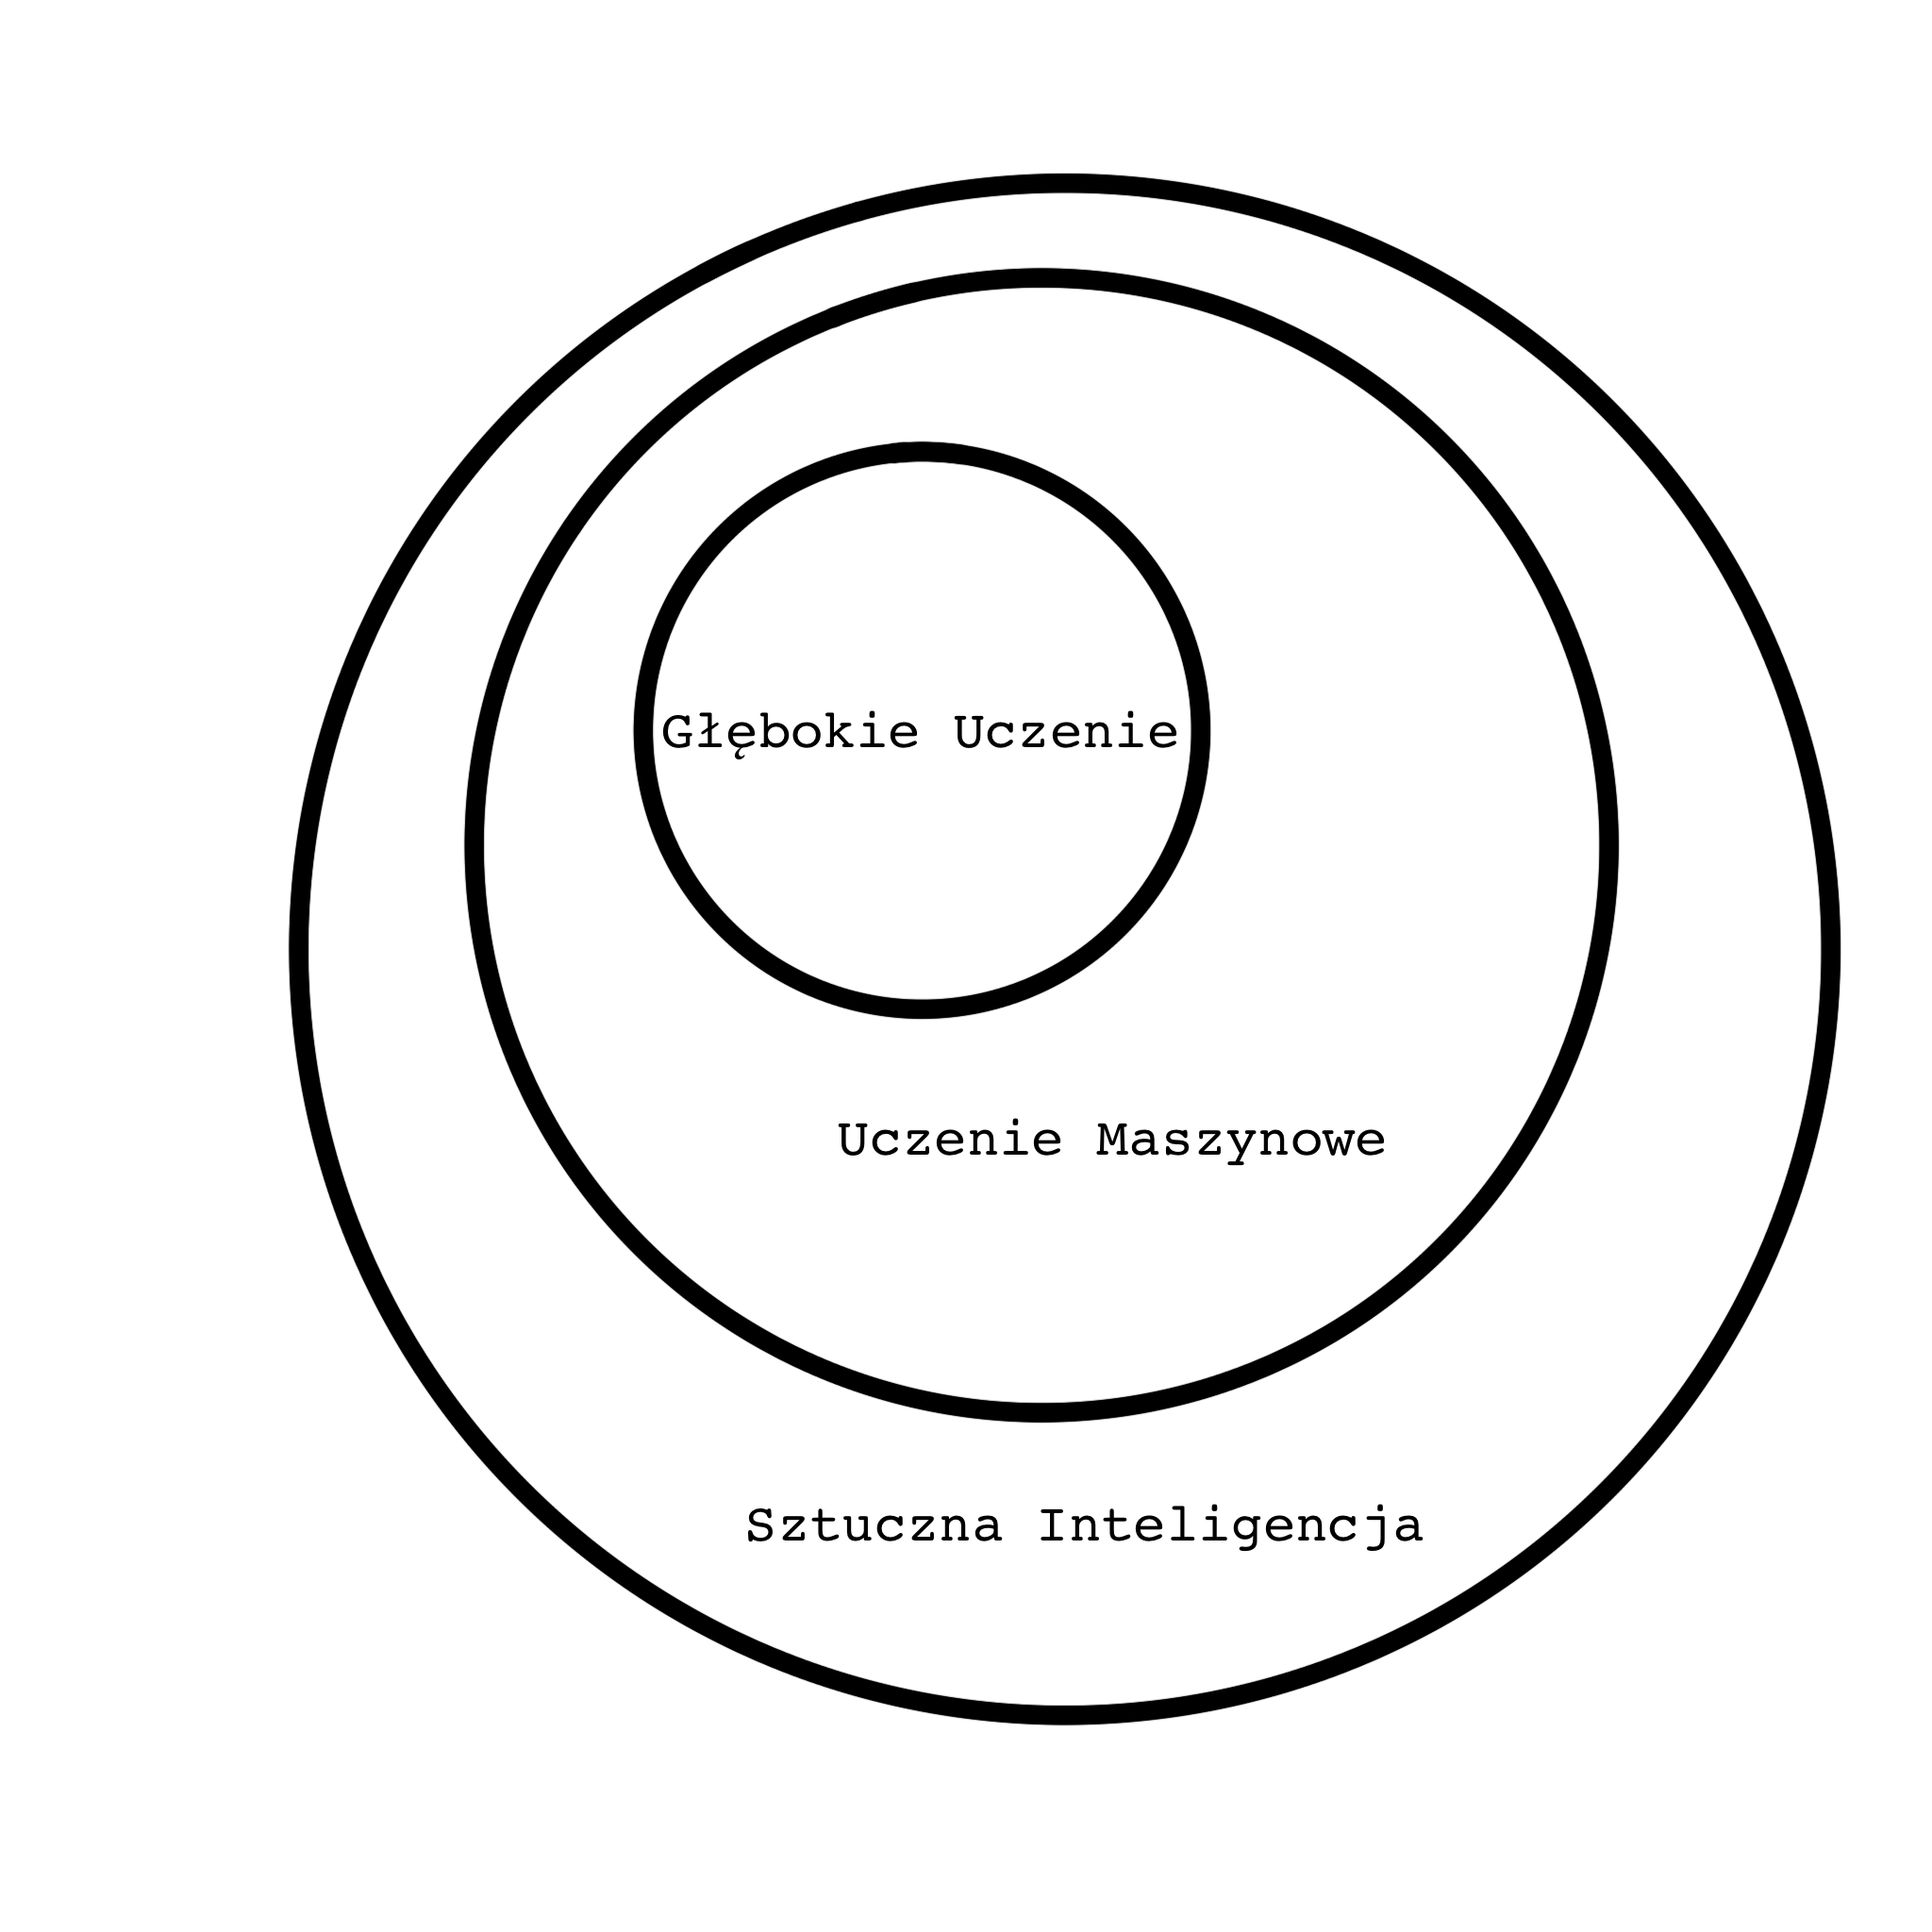
\includegraphics[width=.8\hsize]{fig/1}
\caption{Schemat zawierania pomiędzy głębokim uczeniem, uczeniem maszynowym a sztuczną integencją\label{RYS.1}}
\source{Opracowanie własne}
\end{figure}




\chapter{Sieci Neuronowe  }

napisać, że uczenie maszynowe można zrealizować na x sposobów, jednym z nich są sieci neuronowe. Sieci neuronowe są inspirowane działaniem ludzkiego mózgu itd. W tym rozdziale zostanie omówione to i to, a następnie przedstawione to i tamto.


\section{Neuron  \label{s:dsssl}}
Neuronem określamy najbardziej elementarną cząstkę modelu uczenia maszynowego, często jest to pojedyncza liczba np. odcień szarości (ang. Grayscale Value) dla pojedynczego piksela w przypadku czarno-białego obrazka. Neuron jest podstawowym budulcem sieci neuronowej. 

Powtarzasz w dwóch miejscach, że jest to elementarny element modelu. Dodałbym w osobnym zdaniu jakie przykładowe wartości mogą przyjmować. A także dodałbym w jaki sposób neurony są połączone ze sobą.

\section{Definicja\label{s:dsssl}}

Teoretyczny paradygmat struktur matematycznych inspirowany układem synaps i połączeń między nimi w mózgu. Składowymi sieci neuronowych są neurony oraz połączenia między nimi. Sieci neuronowe otrzymują liczbowe dane wejściowe i przekazują liczbowe dane wyjściowe. Może to być np. klasyfikacja, tłumaczenie lub obliczenie.


\section{Konwolucyjne Sieci Neuronowe  \label{s:dsssl}}

Najpierw bym wyjaśnił co to są konwulocyjne sieci neuronowe, a dopiero później wspominał, że tylko one zostaną przedstawione w pracy.

W tej pracy uwaga poświęcona będzie tylko konwolucyjcym sieciom neuronowym (ang. Convolutional Neural Network), które sprawdzają się przy analizie obrazów.  
Mogą być automatycznie dostosowywane, aby specjalizować się w danym problemie.
Sieci konwolucyjne poprzez trening są w stanie nauczyć się, jakie cechy szczególne obrazu pomagają w jego klasyfikacji. Jest to możliwe dzięki zastosowaniu filtrów badających relacje pikselli będących w sąsiedztwie. Warto jednak wspomnieć o innych sieciach np. Long short-term memory network, które swoje zastosowanie ma w analizie dźwięku. Konwolucyjna sieć neuronowa składa się z jednej lub wielu warstw klastrów połączeń.






\section{Przykład  \label{s:dsssl}}

Posłużmy się przykładem prostej sieci neuronowej, która ma za zadanie rozpoznać pisane cyfry. Jest to swego rodzaju “Hello, World! ” w dziedzinie uczenia maszynowego.
W przypadku analizy obrazka 64x64 piksele jedna warstwa sieci neuronowej sieć neuronowa składać będzie się z 4096 neuronów.

Dlaczego będzie składać się z 4096 neuronów akurat? Napisz z czego to wynika.

Jest to swego rodzaju "Hello, World!" - trochę zbyt potocznie. Nie udziwniałbym i napisał po prostu, że jest to najbardziej elementarny przykład.


Czym jest największa wartość aktywacji? Najpierw wytłumacz, później korzystaj. Wrzuciłbym te wszystkie pod-definicje do podrozdziału "Definicja", gdzie tłumaczysz. I po prostu dałbym od myślnika: Na sieci neuronowe składają się: - neurony - podstawowa ..., - funkcja aktywacji - funkcja, która określa.... I ewentualnie później je bardziej szczegółowo rozwinął.


\begin{figure}[!tbh]
\centering
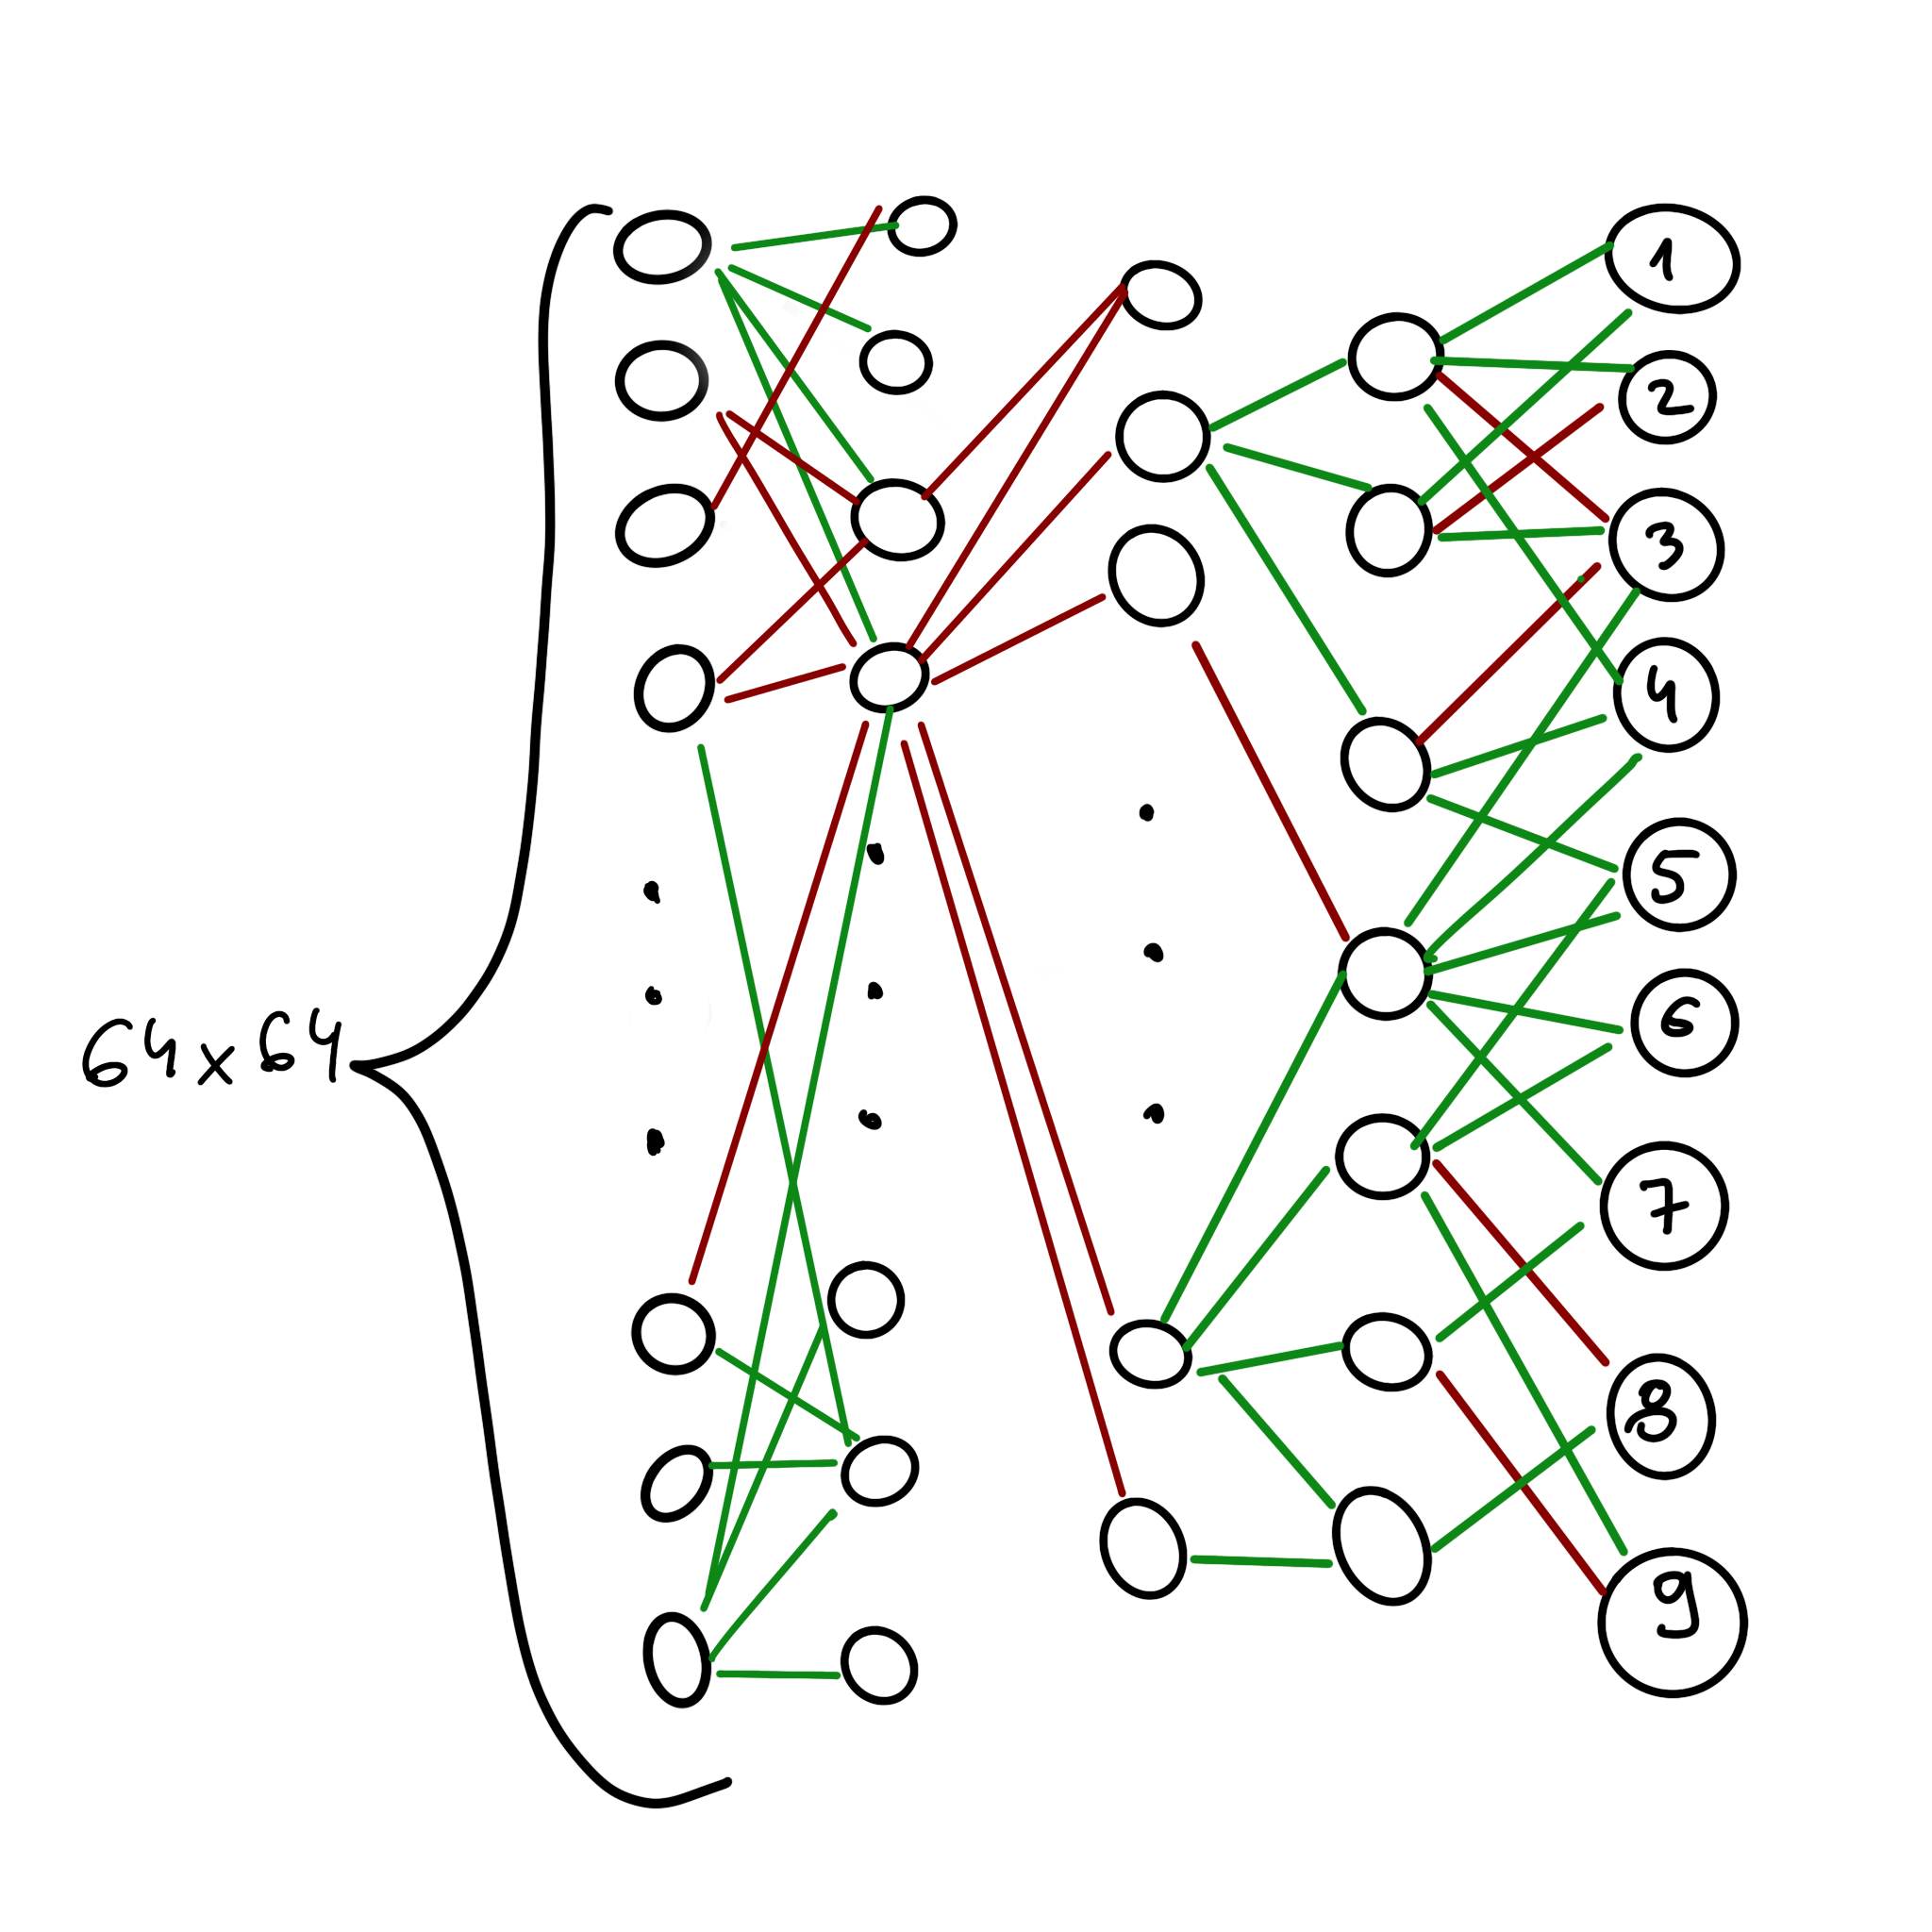
\includegraphics[width=.8\hsize]{fig/2}
\caption{Układ neuronow dla obrazka 64x64 px\label{RYS.2}}
\source{Opracowanie własne}
\end{figure}



Ostatnią warstwą jest output cyfr 0 - 10 i ta z największą wartością aktywacji zostaje wybrana. 

Dokładniej mówiąc neuron to funkcja, która przyjmuje dane wejściowe ze wszystkich neuronów z poprzedniej warstwy i przetwarza to na wartość od 0 do 1, 0 to czarny 1 to biały wartość ta zwana jest “aktywacją” lub “funkcją aktywacji”.

\section{Funkcja aktywacji  \label{s:dsssl}}

Najprostszą jednostką w (głębokich) sieciach neuronowych jest operacja liniowa (skalowanie + przesuwanie), po której następuje funkcja aktywacji.

\begin{figure}[!tbh]
\centering
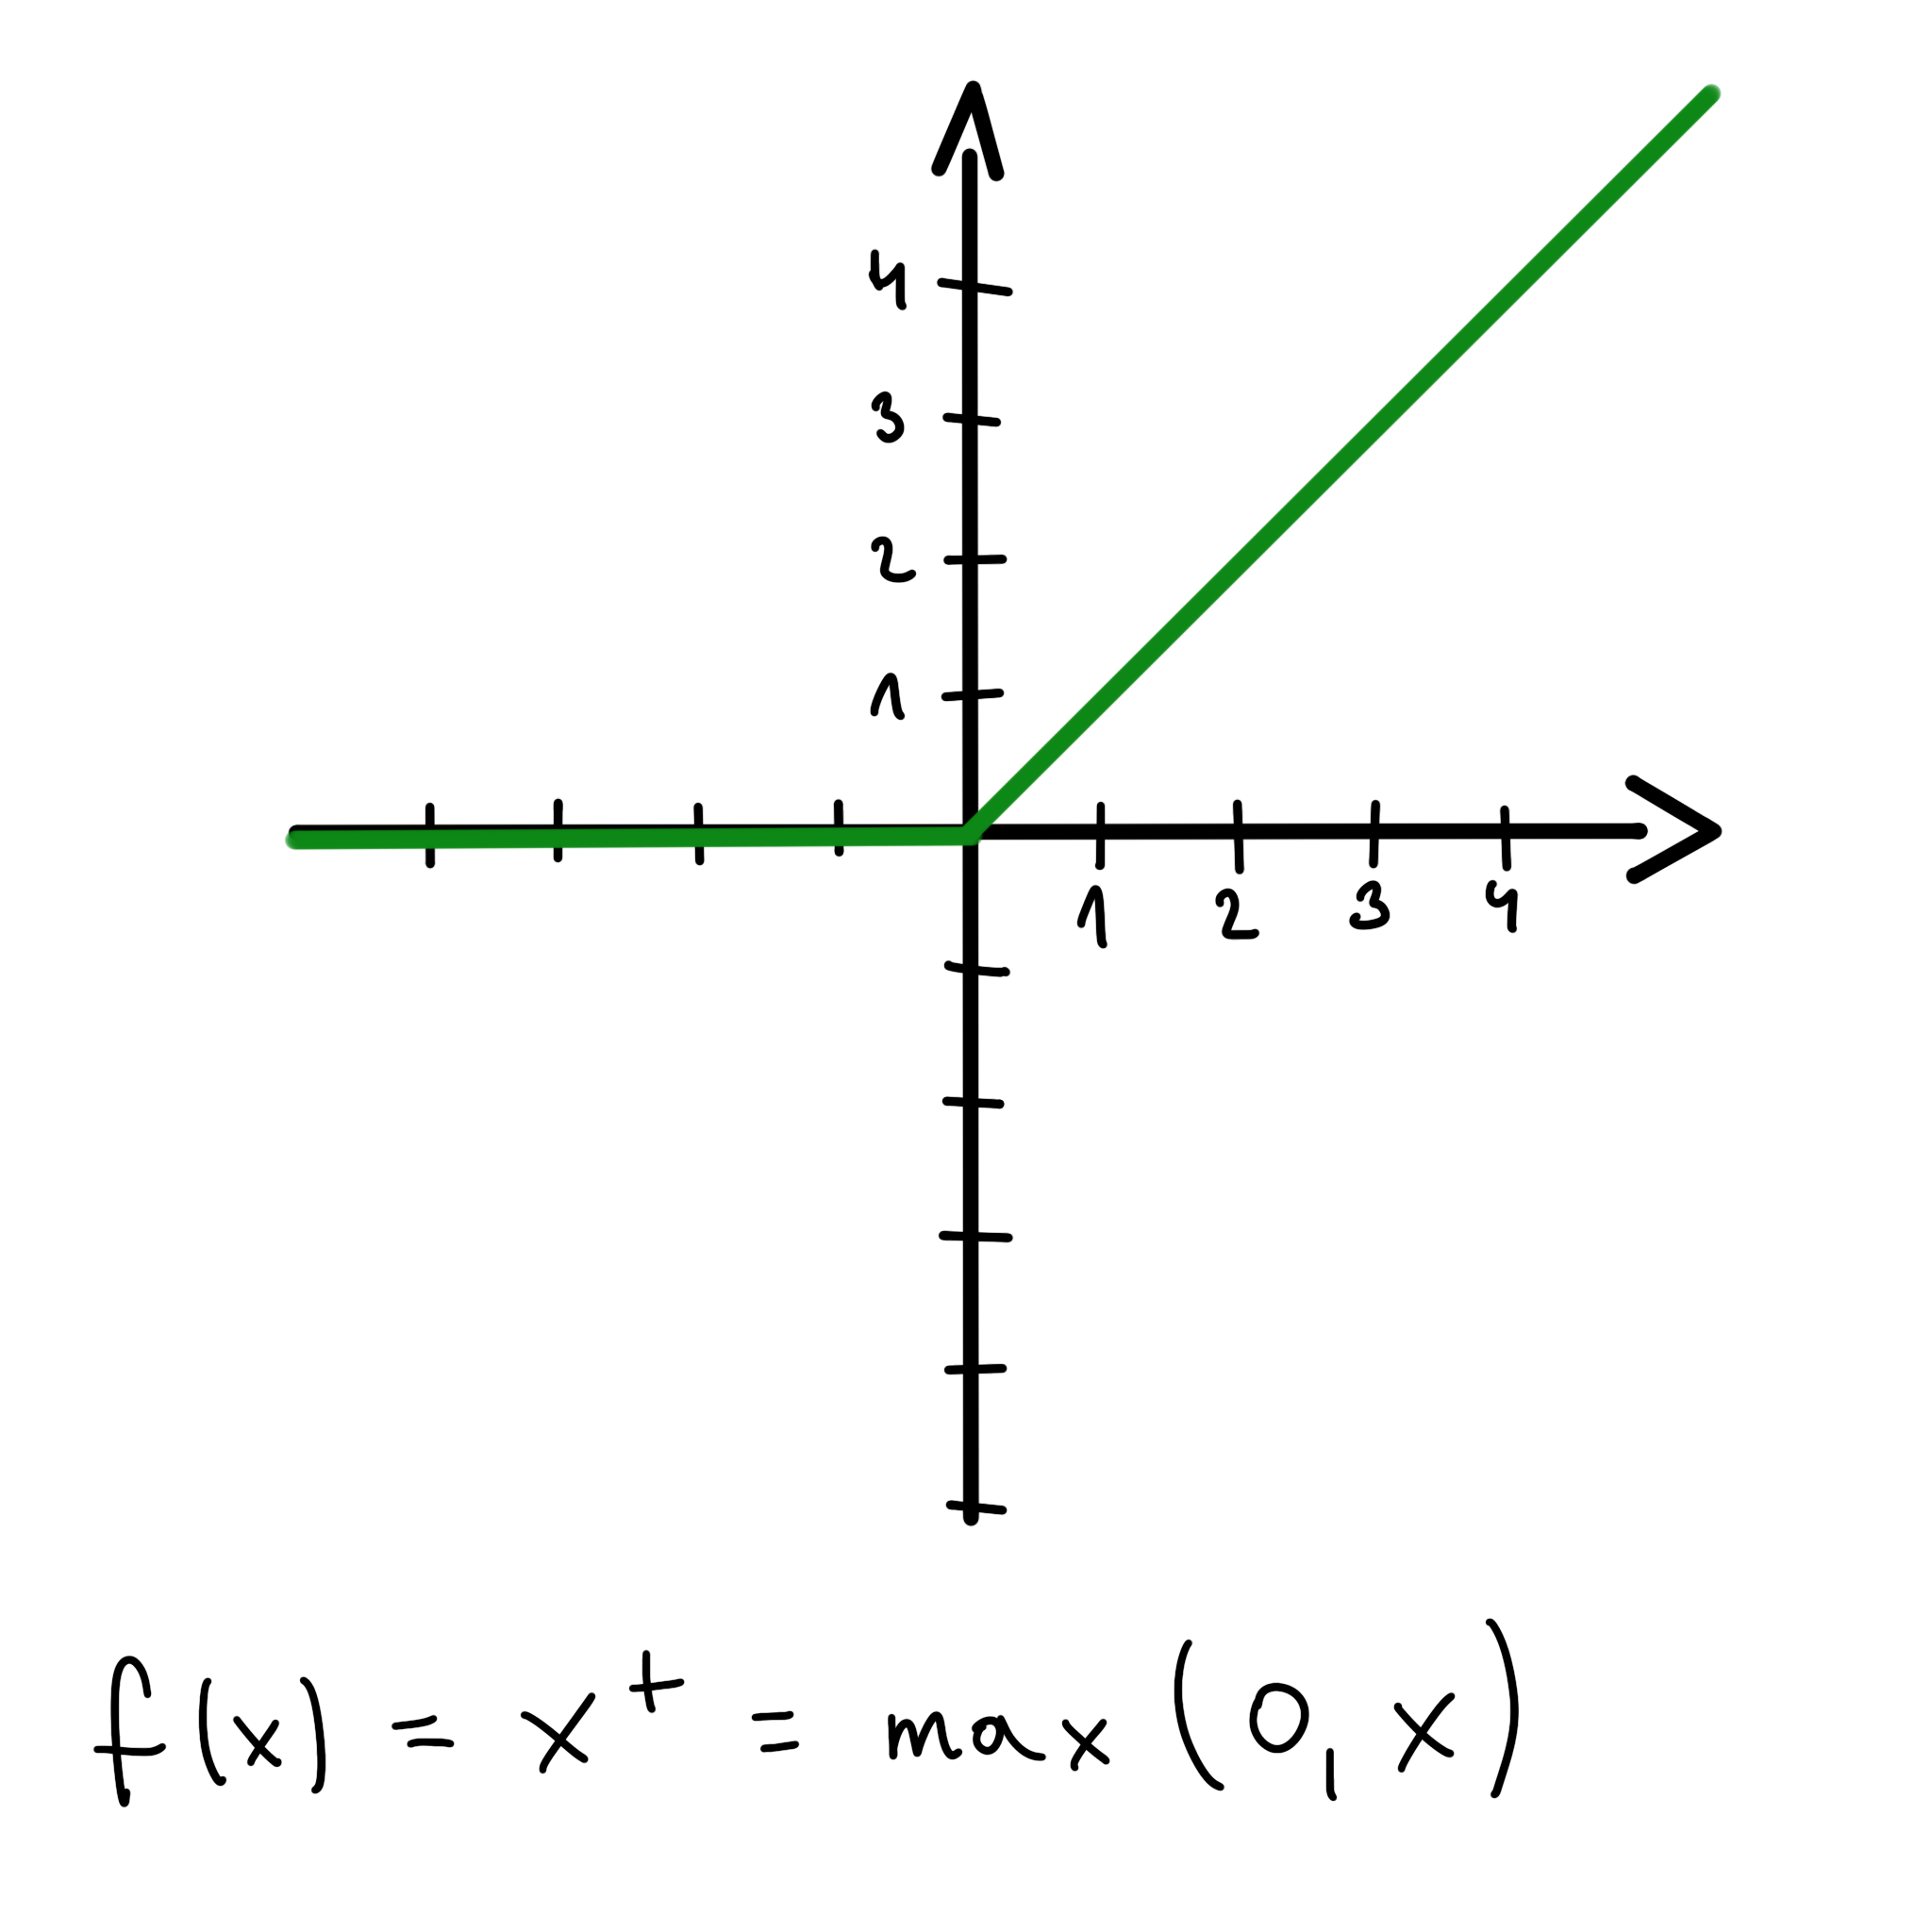
\includegraphics[width=.8\hsize]{fig/4}
\caption{Funkcja ReLU\label{RYS.3}}
\source{Opracowanie własne}
\end{figure}

Funkcja aktywacji ma na celu skoncentrowanie wyników poprzedniej operacji liniowej w danym zakresie.
Aktywacja z poprzedniej warstwy, determinuje aktywację w kolejnych aż do samego końca. 
Dla każdego neuronu wykonywana jest operacja matematyczna:

\begin{equation}
neuron  = φ (w * x + b)
\end{equation}



 Zmienna “x” jest wkładem do obliczeń pojedynczego neuronu , w przypadku rozpoznawania cyfr x jest wartością 0 - 1 odcieniem szarości dla danego piksela, “w” jest wagą, natomiast b to odchylenie.
 
 
 Dodawane jeszcze jest odchylenie (bias), który mówi, jak wysoka musi być suma ważona, zanim neuron zacznie być znacząco aktywny.
 
 
  Objaśnienia wzoru dałbym od myślników. I dodałbym wyjaśnienie - odchylenie od czego?

W każdej warstwie  wartość w neuronie po dodaniu odchylenia i przemnożeniu przez wagę w celu identyfikacji tylko “ważnych” wartości całość przeliczamy jeszcze przez funkcję aktywacyjną. 
Tak zwana warstwa ReLU usuwa ujemne wartości z mapy aktywacji, ustawiając je na zero, co zwiększa nieliniowe właściwości funkcji decyzyjnej i całej sieci.




Dane są często dzielone na osobne zestawy próbek szkoleniowych i próbek walidacyjnych, co pozwala na ocenę modelu na podstawie danych, na których nie był szkolony.


\section{Waga i odchylenie \label{s:dsssl}}
Jest to wartość, która na swój sposób określa jak istotny danych neuronów w przypadku rozpoznawania cyfr pisanych piksele na skraju obrazka będą miały mniejsze znaczenie niż te w okolicach jego centrum. Wagi mówią, jaki wzór pikselowy odbiera neuron w kolejnej warstwie.

Ponownie, dałbym wcześniej - przy okazji objaśniania wzoru.

\begin{figure}[!tbh]
\centering
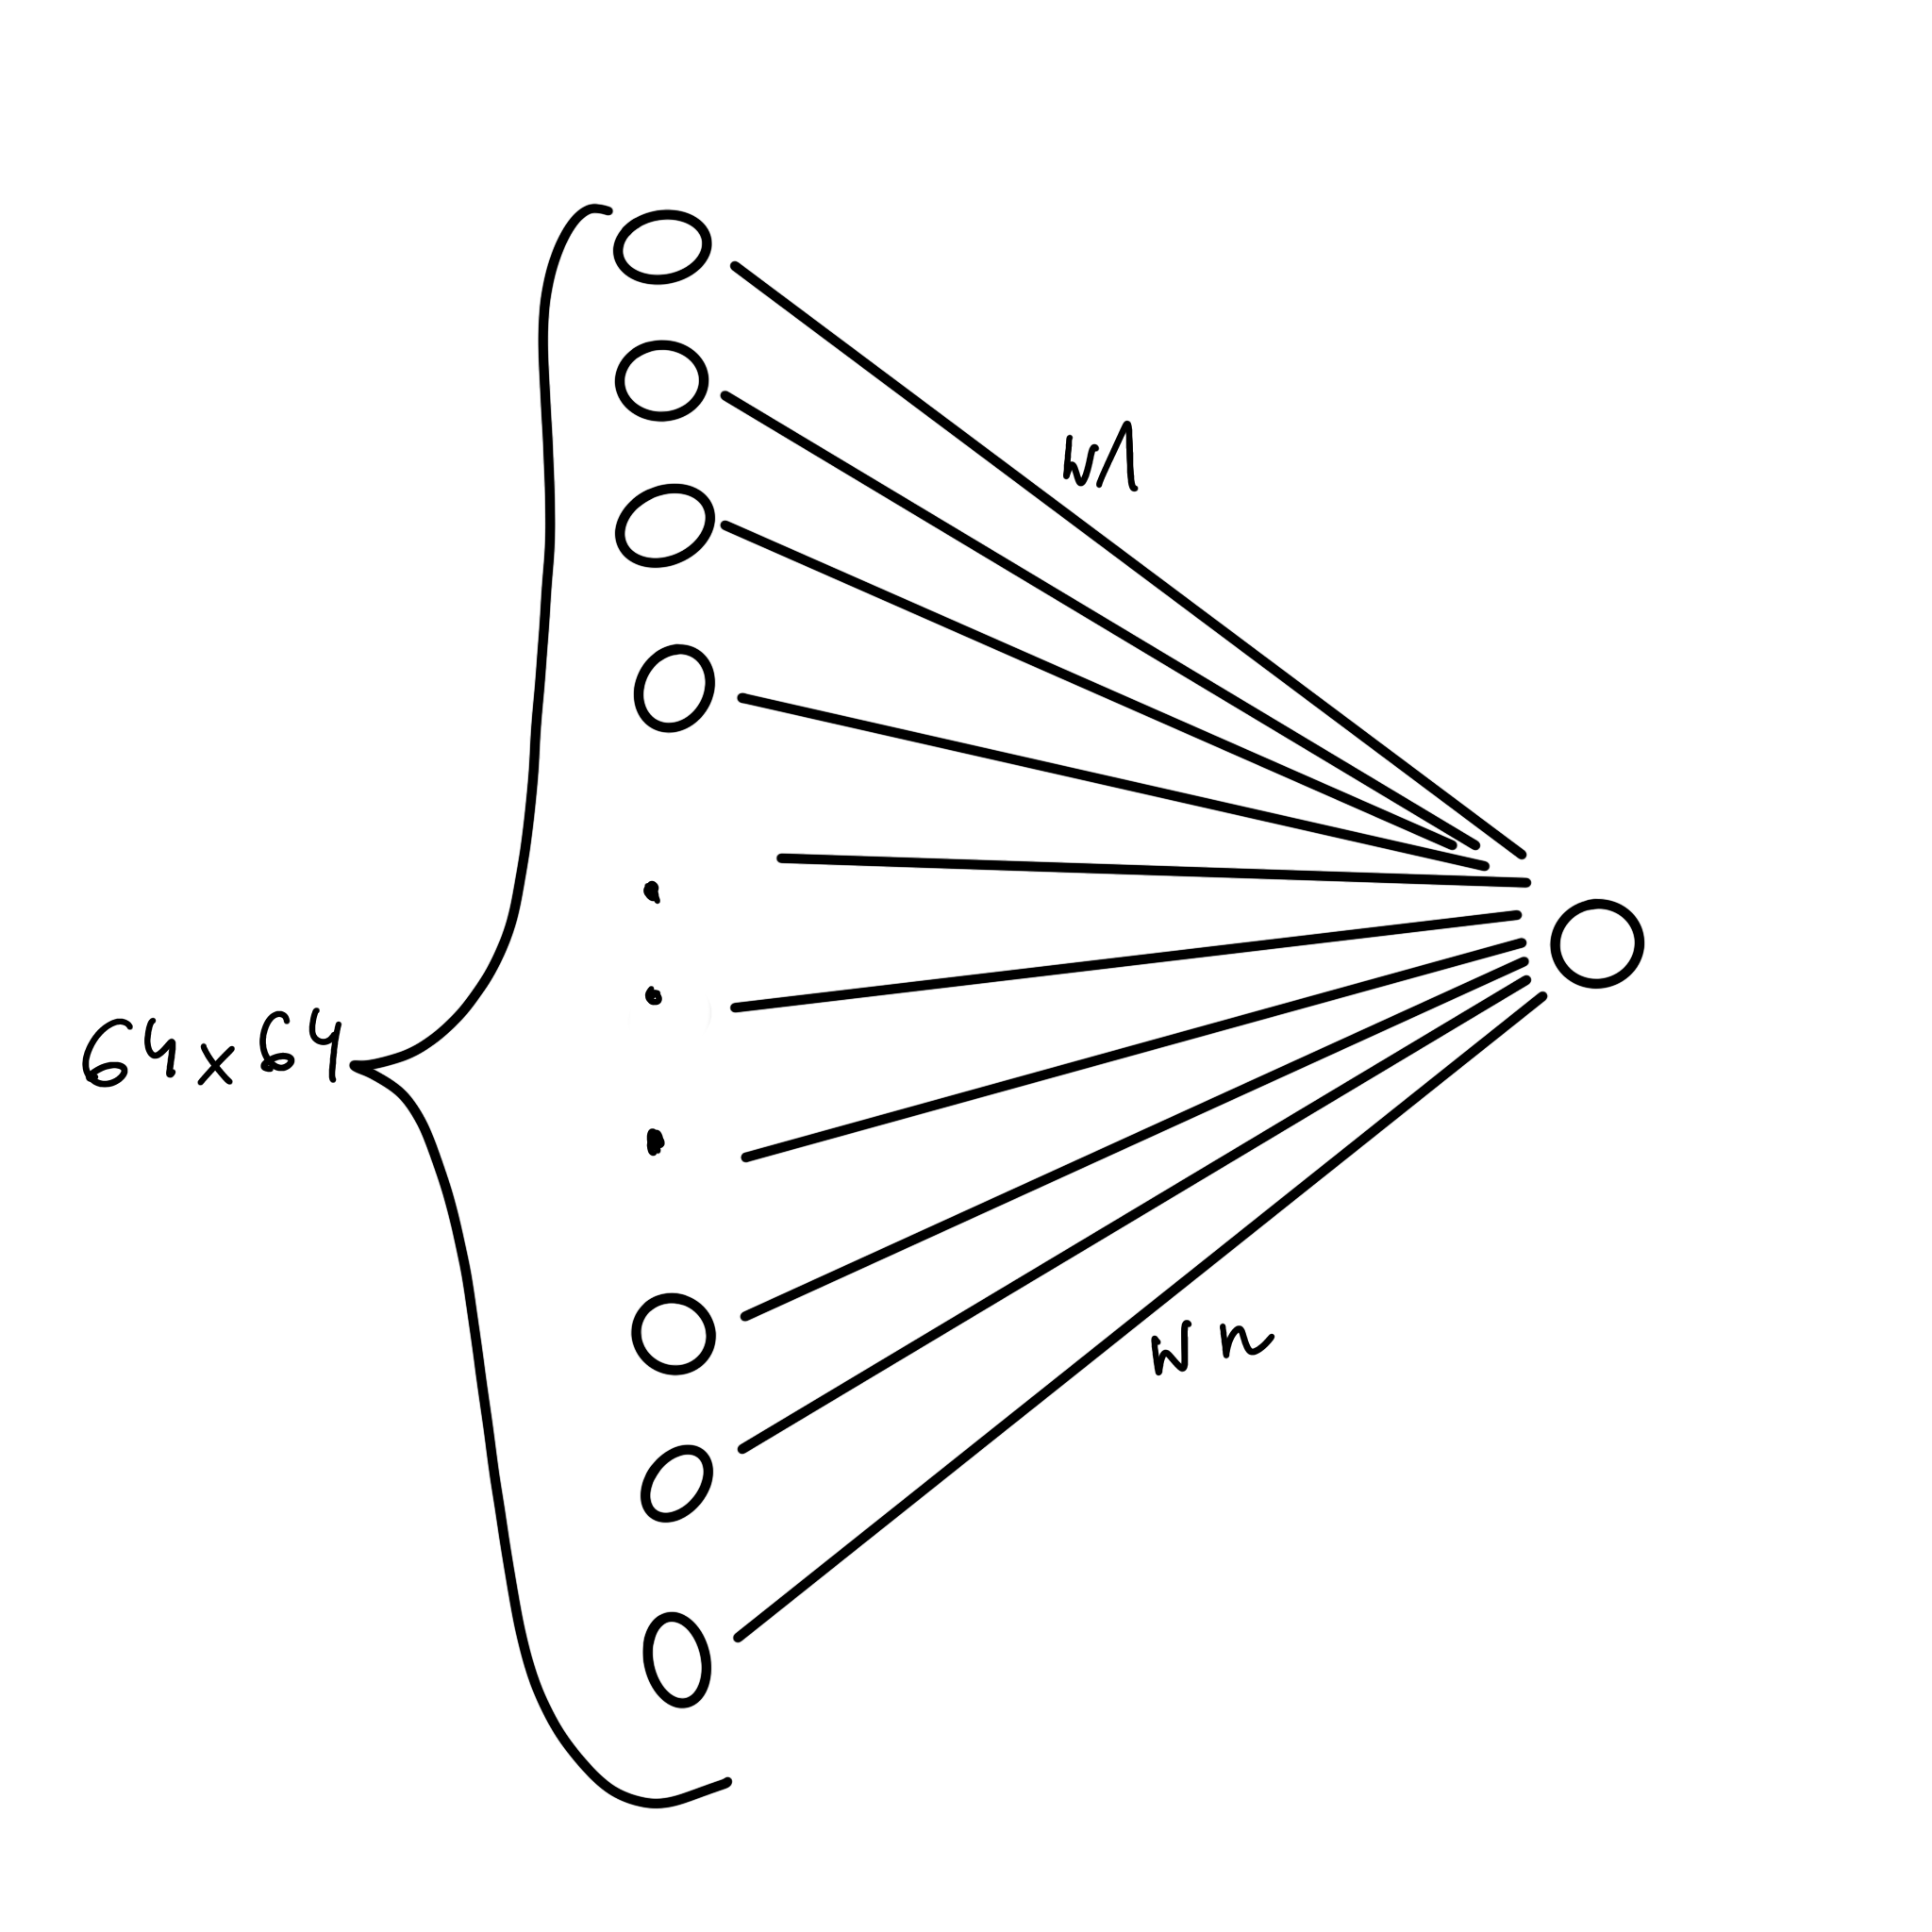
\includegraphics[width=.8\hsize]{fig/3}
\caption{Przypisywanie wag\label{RYS.3}}
\source{Opracowanie własne}
\end{figure}


 Wagi mnożymy z aktywacją ,  aby wagi pomagały w określeniu stopnia aktywacji, zachowujemy je w przedziale od 0 do 1.
 
 \section{Funkcja strat \label{s:dsssl}}
Funkcja strat (ang. loss function) to miara błędu w wykonywaniu zadania, takiego jak błąd między przewidywanymi wyjściami a mierzonymi wartościami. Celem jest, aby funkcja straty była jak najniższa.
 
 \section{Metoda Gradientu Prostego\label{s:dsssl}}

Opracowany przez Cauchy'ego w 1847 r. [6] iteracyjny algorytm optymalizacji pierwszego rzędu do znajdowania lokalnego minimum funkcji różniczkowalnej. Aby znaleźć lokalne minimum funkcji za pomocą opadania gradientu, wykonujemy kroki proporcjonalne do ujemnego gradientu (lub przybliżonego gradientu) funkcji w bieżącym punkcie. Ale jeśli zamiast tego podejmujemy kroki proporcjonalne do dodatniego gradientu, zbliżamy się do lokalnego maksimum tej funkcji; procedura jest wówczas nazywana wynurzaniem gradientowym. 

Dodałbym objaśnienie po co w ogóle mamy zastosować tą metodę. Na co nam znajdowanie lokalnych minimów


\begin{equation}
optimizer = optim.Adam()
\end{equation}


Objaśnienia do wzoru, co robi optim.Adam()? 

Im więcej kroków optymalizacji tym bardziej efektowny będzie transfer stylu.


\section{Wsteczna Propagacja\label{s:dsssl}}

W uczeniu maszynowym propagowanie wsteczne (ang. backpropagation) jest szeroko stosowanym algorytmem w uczeniu sieci neuronowych przekazywanych do nadzorowanego uczenia. Przy dopasowywaniu sieci neuronowej propagacja wsteczna oblicza gradient funkcji utraty w odniesieniu do wag sieci dla przykładu z pojedynczym wejściem i wyjściem i robi to skutecznie, w przeciwieństwie do naiwnego bezpośredniego obliczania gradientu w odniesieniu do każdej masy indywidualnie. Ta wydajność umożliwia stosowanie metod gradientowych do szkolenia sieci wielowarstwowych, aktualizując wagi w celu zminimalizowania strat. Algorytm wstecznej propagacji działa poprzez obliczenie gradientu funkcji utraty w odniesieniu do każdej masy według reguły łańcuchowej, obliczanie gradientu pojedynczej warstwy na raz, iterowanie wstecz od ostatniej warstwy.

Brakuje właśnie informacji, po co nam ta propagacja i metoda z poprzedniego podrozdziału. Dodałbym omówienie tego we wstępie do rozdziału.




 \section{Podsumowanie \label{s:dsssl}}
 
Podsumowując można uważać za  poprawne stwierdzenie, iż uczenie się sieci to tylko modyfikowanie wag oraz odchyleń tak, aby osiągać najlepsze rezultaty, czyli uczenie się jest swego rodzaju oszacowaniem parametrów.   

 Warto dodać iż często w przypadku gdy sieć neuronowa ma rozpoznawać zależności bazujące na kształtach a rozpoznawanie cyfr pisanych właśnie takie jest, często redukuje się dane wejściowe do minimum. Zamienia się wtedy kolorowy obrazek RGB na czarno-biały. Dzięki takiemu zabiegowi sieć neuronowa nie jest zaśmiecona niepotrzebnymi dany jakim jest kolor i może to dać lepszą rozpoznawalność jak również wzrost wydajności zarówno w procesie szkolenia jak i działania klasyfikatora.  
 
 "zaśmiecona" to potoczne określenie


\chapter{Widzenie komputerowe  }


Możliwośc interpretacji i przetwarzania obrazu przez programy zostało zrewolucjonizowane
przez wprowadzenie konwolucyjnych sieci neuronowych, a systemy oparte na obrazach zyskały nowy zestaw możliwości. 

Rozdział ten traktować będzie o możliwościach odczytu przetwarzania oraz zapisu opbrazów.

Trochę nie trzyma się to kupy - najpierw piszesz, że zostały zrewolucjoniowane przez wprowadzenie sieci neuronowych i nagle urywasz temat pisząc o czym będzie ten rozdział. Nie pisałbym o poprzednim rozdziale (jeśli treść nie jest powiązana), a jeśli jest to napisałbym dlaczego o tym wspominasz. No i znowu opisałbym co będzie omówione w tym rozdziale, po co nam widzenie komputerowe, może definicje najważniejszych pojęć.

 \section{RGB\label{s:dsssl}}
 Istnieje kilka sposobów kodowania liczb na kolory. Najczęstszym jest
RGB, który określa kolor za pomocą trzech liczb reprezentujących intensywność czerwieni, zieleni i niebieskiego. 

Jaki obrazek? 

W tym momencie obrazek jest obiektem podobnym do tablicy o trzech wymiarach: dwóch wymiarach przestrzennych (szerokość i wysokość) i trzecim wymiarze odpowiadającym kanałom czerwonym, zielonym i niebieskim. 

Każdy kolor będzie reprezentowany jako 8-bitowa liczba całkowita, jak w większości formatów fotograficznych ze standardowych aparatów konsumenckich.

Sieci neuronowe zwykle działają z wejściowymi tensorami zmiennoprzecinkowymi. Sieci neuronowe wykazują najlepszą wydajność treningu, gdy dane wejściowe mieszczą się w przedziale od około 0 do 1 lub –1 do 1 (efekt definiowania ich bloków konstrukcyjnych). Sieci neuronowe wymagają przedstawienia danych jako wielowymiarowych tensorów numerycznych, często 32-bitowych liczb zmiennoprzecinkowych.

Powtarzasz za często "Sieci neoronowe". Trochę też zbyt dynamicznie zmieniasz temat. Najpierw piszesz o RGB, a nagle o sieciach neuronowych. I jest takie wtf, kiedy przeszedłem do innego rozdziału. Połącz jakoś te tematy - Wykorzystanie rgb w sieci neuronowych ... coś wtym rodzaju.


Typową rzeczą, którą należy zrobić, jest rzutowanie tensora na zmiennoprzecinkowe i normalizacja wartości pikseli. Rzutowanie na zmiennoprzecinkowe jest łatwe, ale normalizacja jest trudniejsza, ponieważ zależy od tego, jaki zakres danych wejściowych, który zdecydujesz, powinien wynosić od 0 do 1 (lub –1 do 1). Jedną z możliwości jest podzielenie wartości pikseli przez 255 (maksymalna reprezentowana liczba w 8-bitowym znaku bez znaku):


Nie za bardzo wiem - jaki jest cel tego podrozdziału. Tzn. nagłówek jest RGB, a w środku najpierw faktycznie tłumaczysz co to jest rgb, ale następnie piszesz o sieciach neuronowych. Oddzieliłbym to na osobny podrozdział, albo zrobił jakieś płynne przejście. 

Po załadowaniu jednego z popularnych formatów obrazów, a należy przekształcić dane w reprezentację tensora, która ma różne części obrazu ułożone w sposób zgodny z oczekiwaniami danego API uczenia maszynowego.

To zdanie trzeba przebudować, bo jest ciężkie do czytania.

\section{Tensor\label{s:dsssl}}
Tensor[4], jest to wielowymiarowa tablica. Sieci neuronowe pobierają tensory na wejściu i wytwarzają tensory jako wyjścia. W rzeczywistości wszystkie operacje w sieci neuronowej i podczas optymalizacji są operacjami między tensorami, a wszystkie parametry (takie jak wagi i odchylenia) w sieci neuronowej są tensorami.

Ponownie mieszasz definicje z wykorzystaniem. Najpierw tłumaczysz, że to wielowymiarowa tablica, później dajesz wykorzystanie w sieciach neuronowych, a dalej znowu piszesz co to jest.

Tensor to struktura danych przechowująca zbiór liczb, które są dostępne indywidualnie za pomocą indeksu i które mogą być indeksowane za pomocą wielu indeksów.

Termin tensor jest dołączony do pojęcia przestrzeni, układów odniesienia i transformacji między nimi. Dla wszystkich innych tensor odnosi się do uogólnienia wektorów i macierzy do dowolnej liczby wymiarów, jak pokazano na rysunku.
Tensor reprezentujące wartości w poszczególnych pikselach są często kodowane za pomocą liczb 8-bitowych, na przykład w kamerach konsumenckich. W zastosowaniach medycznych, naukowych i przemysłowych nierzadko można znaleźć piksele o większej precyzji numerycznej, takie jak 12-bitowe i 16-bitowe.

 Ta precyzja zapewnia szerszy zakres lub zwiększoną czułość w przypadkach, w których piksel koduje informacje dotyczące właściwości fizycznej, takiej jak gęstość kości, temperatura lub głębokość.
 
 \begin{figure}[!tbh]
\centering
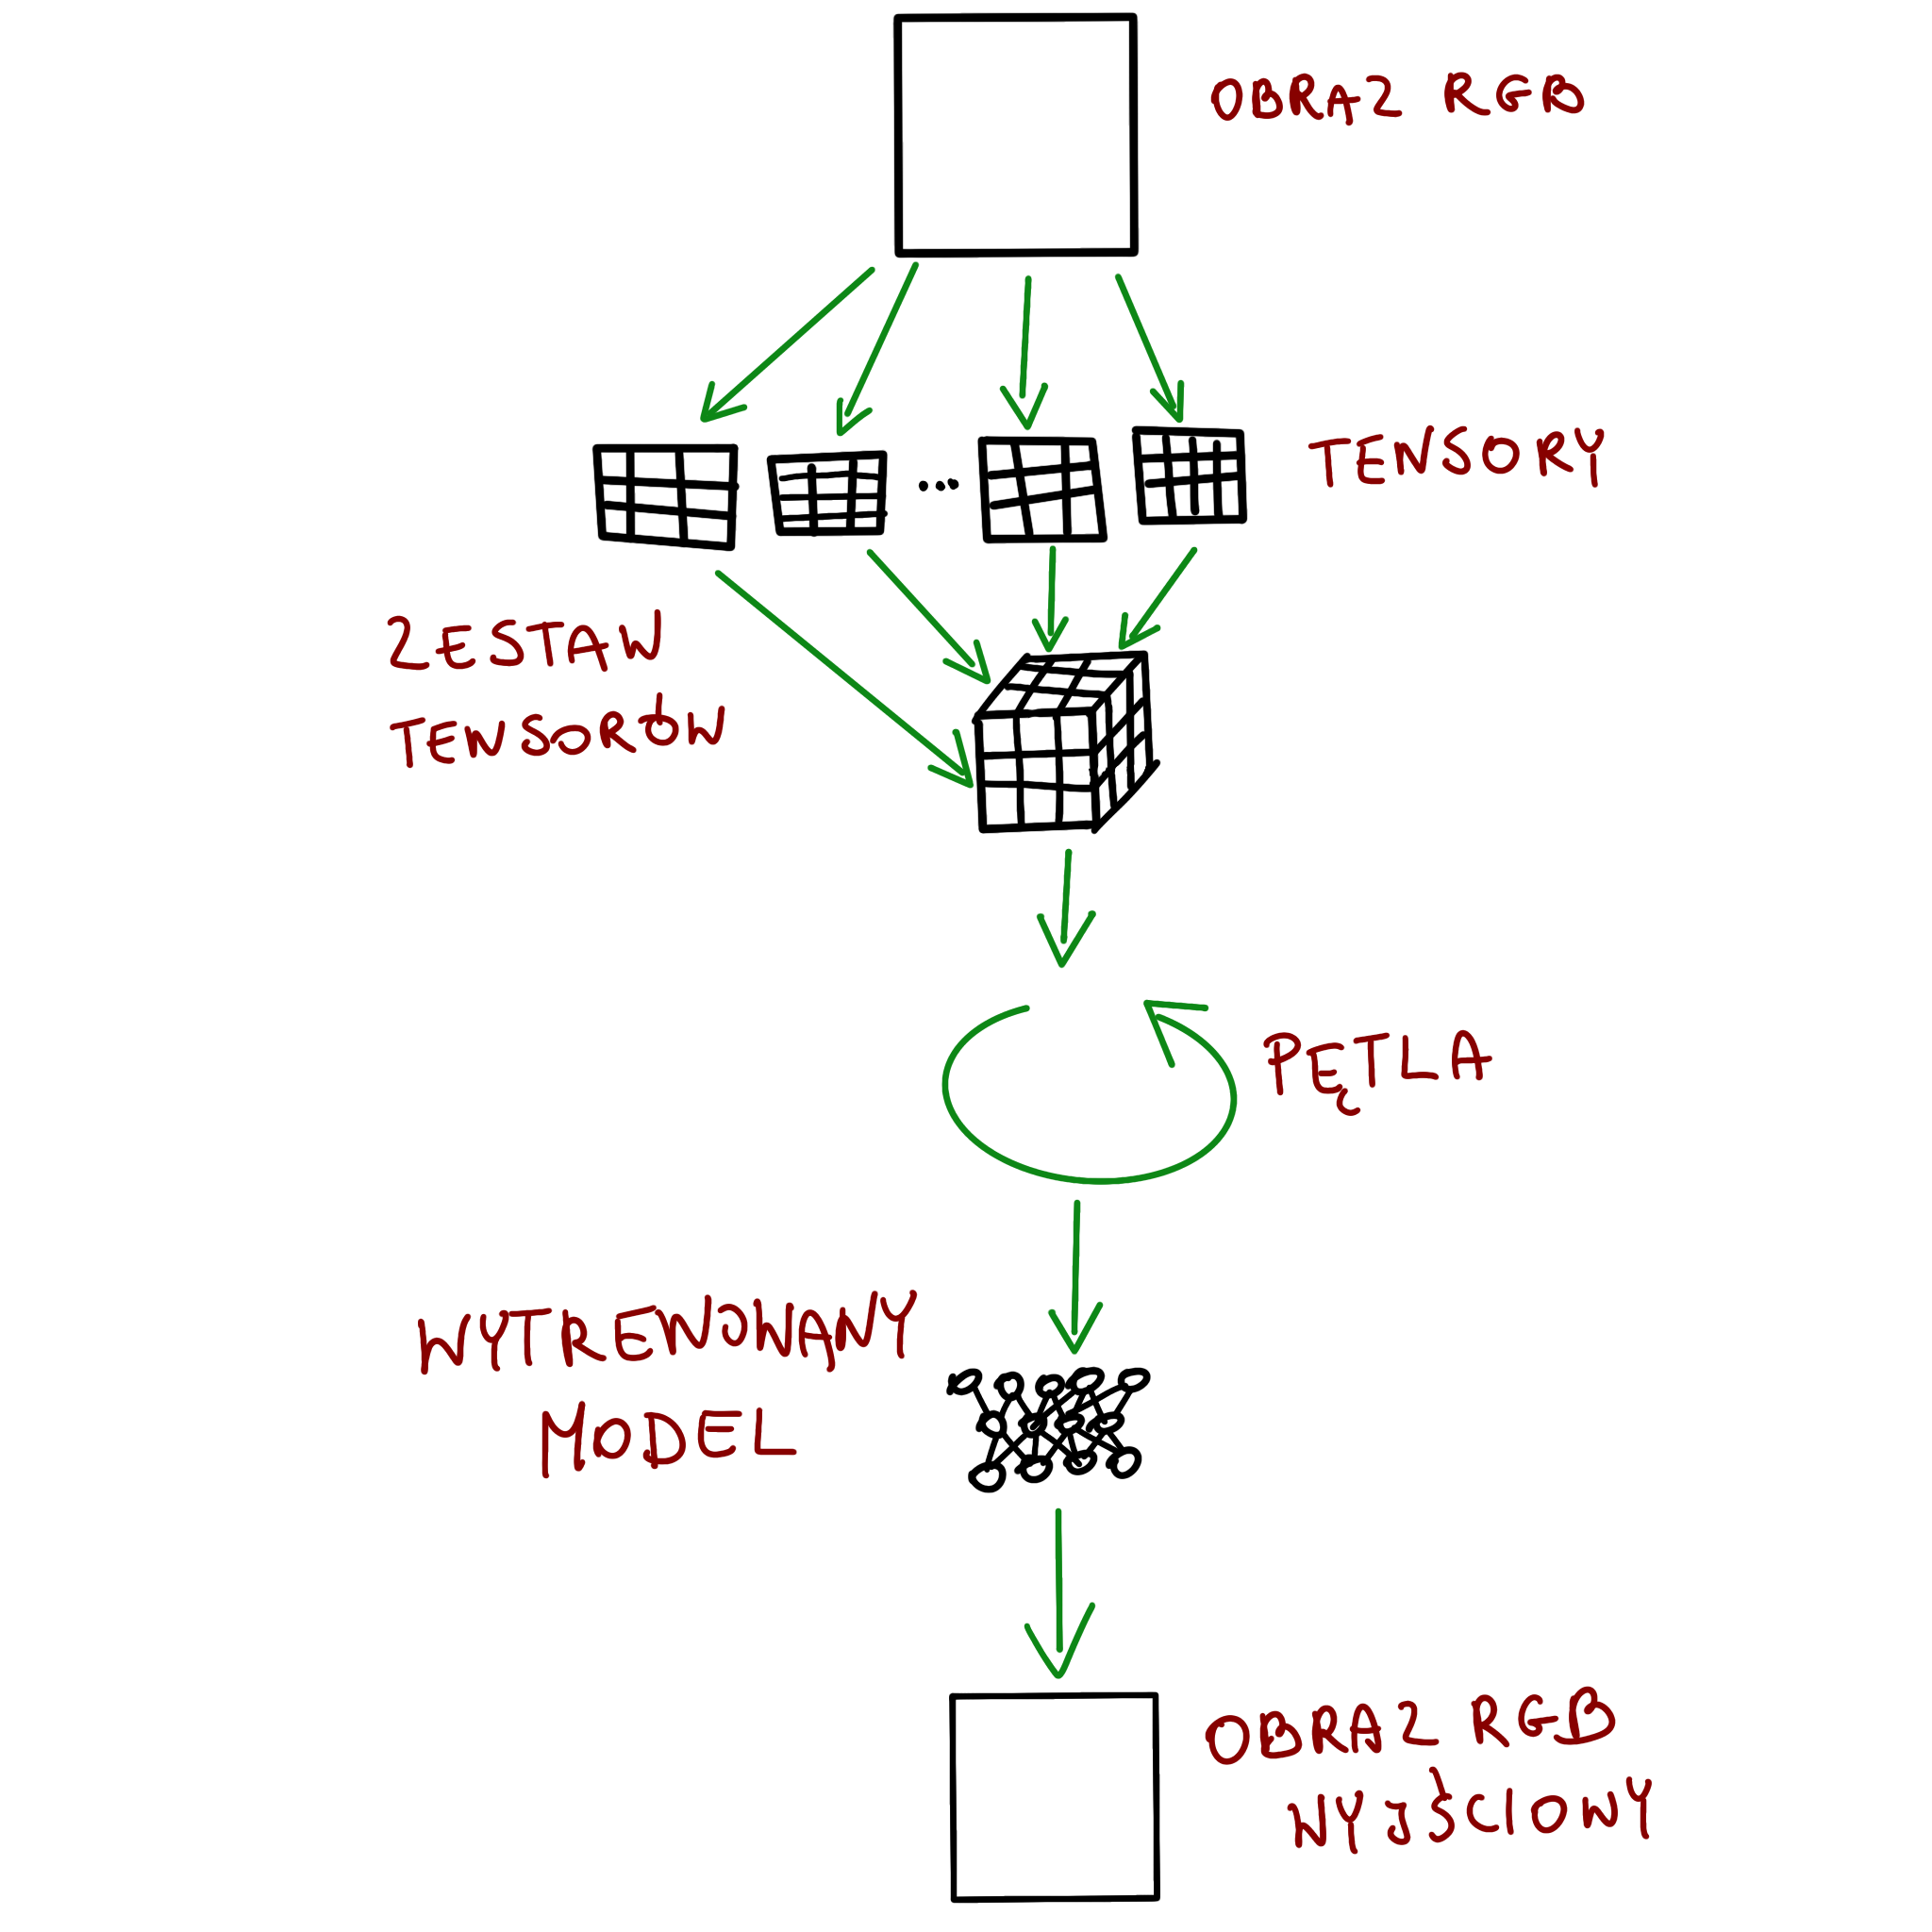
\includegraphics[width=.8\hsize]{fig/5}
\caption{Schemat przetwarzania obrazu\label{RYS.5}}
\source{Opracowanie własne}
\end{figure}

 Dodałbym jakąś wzmiankę w tekscie o tym rysunku -> na rysunku 3.1 został przedstawiony....


 \section{Operacje na tensorach\label{s:dsssl}}
Na tensorach można  wykonać kilka innych operacji na danych wejściowych, w tym przekształcenia geometryczne, takie jak obrót, skalowanie i kadrowanie. Operacje te mogą pomóc w szkoleniu lub mogą być wymagane, aby dowolne dane wejściowe były zgodne z wymaganiami wejściowymi sieci, takimi jak rozmiar obrazu.

Rozwiń ten podrozdział, albo go zmerguj z poprzednim - jest za krótki w stosunku do reszty.


\chapter{Przegląd dostępnych narzędzi}

Ponownie wstęp - po co nam te narzędzia, po co robimy ich przegląd, dlaczego w ogóle ten wybór jest ważny. Po przeczytaniu rozdziału, zmieniłbym nazwę rozdziału - To jest omówienie narzędzi, które zostały wykorzystane, a nie przegląd "dostępnych". Byś musiał pokazać jakie inne narzędzia jeszcze są dostępne, żeby tytuł był adekwatny.

\section{Blender\label{s:dsssl}}

Blender jest to wolnym i otwartym oprogramowaniem do modelowania i renderowania obrazów oraz animacji trójwymiarowych.Pozwala on na pisanie w języku python skryptów, które poszerzają podstawowe funkcjonalności blendera.

\section{Python\label{s:dsssl}}

Język Python powstał już w latach dziewięćdziesiątych, między innymi dzięki rewolucji uczenia maszynowego przeżywa swoją drugą młodość. Cechuje się klarownością kodu źródłowego.
Jest to język, z którego w większości składa się Blender. Każda wersja blendera ma wbudowaną już własną wersję pythona. 

Oszczędziłbym uwag typu "cechuje się klarownością kodu źródłowego", ponieważ co programista to inne zdanie. Możesz napisać, zamiast tego powody, dla którego tak często jest używany przy uczeniu maszynowym.

\section{Wtyczki\label{s:dsssl}}

Jedną z wielu zalet środowiska Blender jest jego otwartość. Większość kodu jest otwarta i konfigurowalna, ułatwia to tworzenie rozszerzeń (wtyczek).



Wtyczki w Blenderze mogą istnieć w postaci pojedynczych skryptów 

\begin{equation}
*.py
\end{equation}

lub zestawu skryptów pakowanych w 
\begin{equation}
*.zip
\end{equation}

.zip. Uruchamiany wtedy jest plik 

\begin{equation}
\_\_init\_\_.py
\end{equation}


Zarówno wtyczki do Blendera jak i same operacje przy użyciu PyTorch’a mogą być tworzone na dowolnym systemie operacyjnym. Te narzędzia znacznie ułatwiają pracę nad tego typu oprogramowaniem.

\begin{figure}[!tbh]
\centering
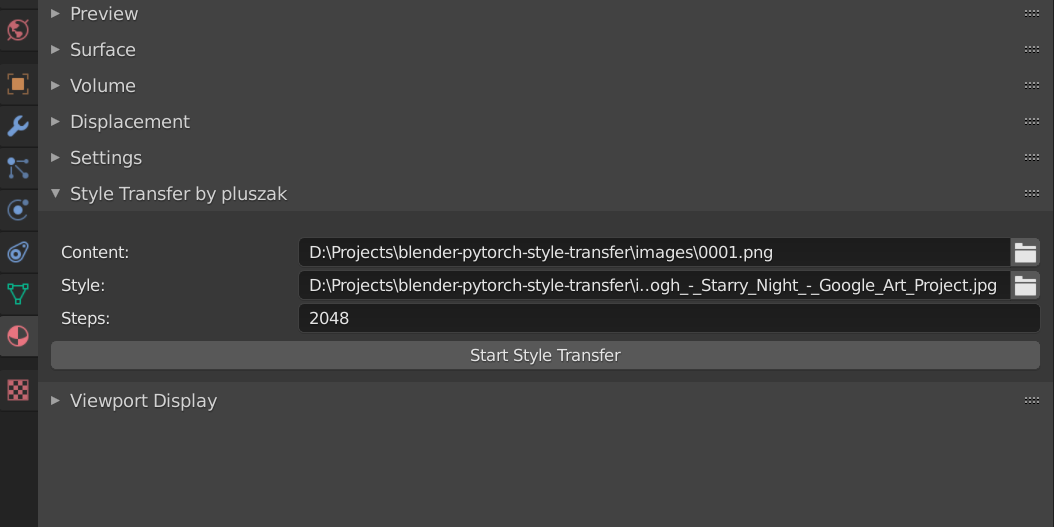
\includegraphics[width=.8\hsize]{fig/9}
\caption{Inplementacja Transferu Stylu jako wtyczki w Blenderze\label{RYS.9}}
\source{Opracowanie własne}
\end{figure}

\section{PyCharm\label{s:dsssl}}
 PyCharm to zintegrowane środowisko programistyczne (IDE) dla języka programowania Python firmy JetBrains. Zapewnia m.in.: edycję i analizę kodu źródłowego, graficzny debugger, uruchamianie testów jednostkowych, integrację z systemem kontroli wersji.
 
 \section{Jupyter Notebook\label{s:dsssl}}
 
Jupyter Notebook to iInteraktywne środowisko pozwalająca na wykonywanie kodu uczenia maszynowego po stronie serwera. Pozwala na szybkie debugowanie i testowanie kodu między innymi biblioteki PyTorch.

 \section{CUDA\label{s:dsssl}}
 
CUDA (ang. Compute Unified Device Architecture) jest to opracowana przez firmę Nvidia uniwersalna architektura procesorów wielordzeniowych (głównie kart graficznych) umożliwiająca wykorzystanie ich mocy obliczeniowej do rozwiązywania ogólnych problemów numerycznych w sposób wydajniejszy niż w tradycyjnych, sekwencyjnych procesorach ogólnego zastosowania. Charakteryzuje się ona wyszszym współczynnikiem FLOPS (ang. floating point operations per second) czyli ilości operacji zmiennoprzecinkowych na sekundę.

Dodałbym do tych wszystkich narzędzi opis w jaki sposób będą one wykorzystane w pracy.


\chapter{Przegląd dostępnych bibliotek}

Ponownie wstęp i tytuł do zmiany.

 \section{PIP\label{s:dsssl}}
 PIP (ang. Package In Python) to standardowy system zarządzania rozszerzeniami i bibliotekami w Pythonie.
 \begin{equation}
python.exe\:-m\:ensurepip
\end{equation}

Wszystkie inne zewnętrzen bibilioteki pythona instalowane są przy pomocy biblioteki PIP.
 
  \section{BPY\label{s:dsssl}}
  
  BPY (ang. Blender Python) to biblioteka do komunikowania się z Blenderem, a konkretnej z Pythonem wbudowanym w Blendera. Wszystkie operacje, które można wykonać przy pomocy intefejsu gragicznego Blendera można też przedstawić jako kod wykonywany przy odwołaniu do BPY.
  
  
  \begin{figure}[!tbh]
\centering
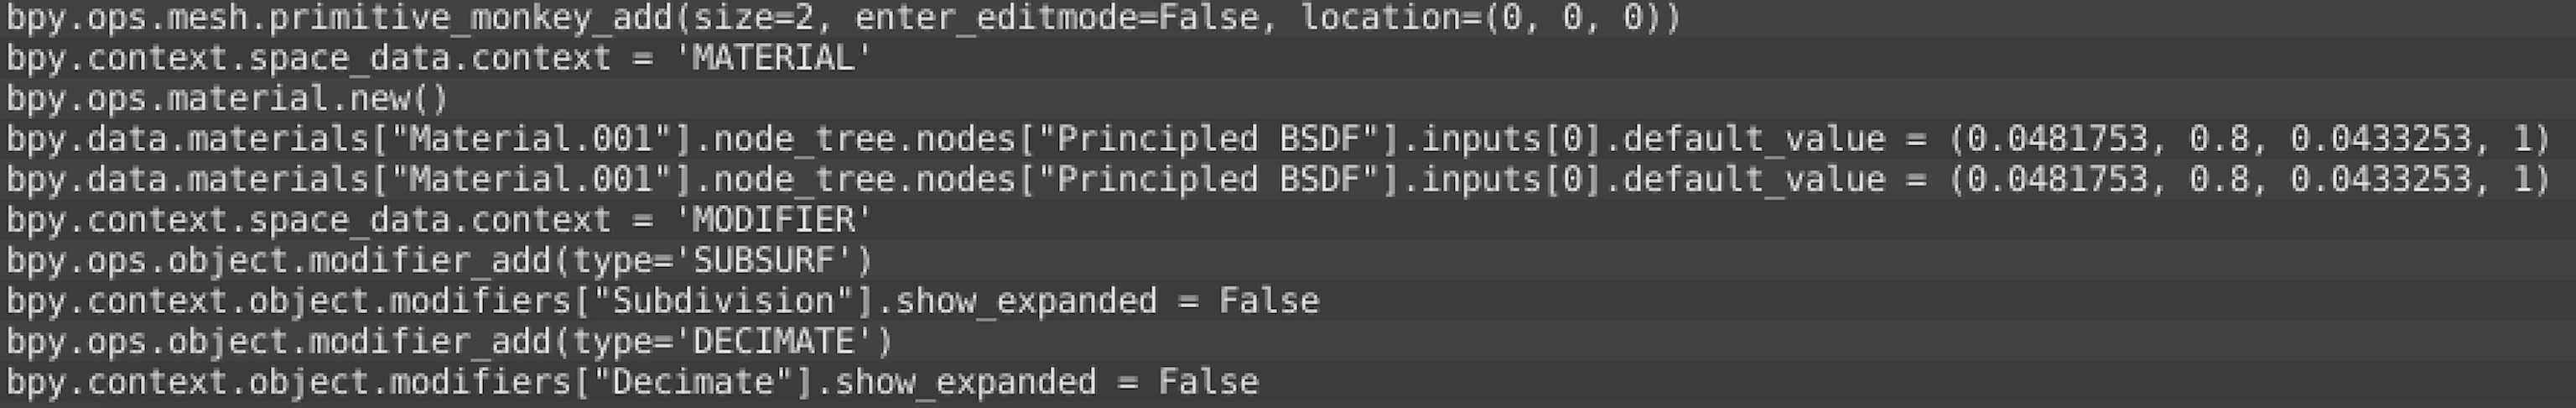
\includegraphics[width=1.2\hsize]{fig/8}
\caption{Przykład prostych operacji w Blenderze, przedstawone w postaci kodu z odwołaniem do BPY. Między innymi znajedzimy tu dodanie nowego materiału, zminę koloru, dodoanie modyfikatora Subdivision.\label{RYS.3}}
\source{Opracowanie własne}
\end{figure}
  
    \section{PyTorch\label{s:dsssl}}
    
    
PyTorch to biblioteka, która ułatwia budowanie projektów głębokiego uczenia się. Podkreśla elastyczność i pozwala wyrazić modele głębokiego uczenia się w idiomatycznym języku Python. Ta przystępność i łatwość użycia znalazły wczesnych użytkowników w społeczności badawczej, a od lat od wydania biblioteki stała się jednym z najważniejszych narzędzi do głębokiego uczenia się dla szerokiego zakresu aplikacji.

Instalujemy ją przy pomocy wcześniej wspomnianego PIP-a:

\begin{equation}
python.exe\:-m\:pip\:install\:torch
\end{equation}

Dzięki integracji bibliotek PyTorch ze standardową biblioteką Python i otaczającym ekosystemem, ładowanie najpopularniejszych rodzajów danych i konwertowanie ich do tensorów PyTorch jest wygodne.􏰹Biblioteki takie jak PyTorch pozwalają efektywnie budować i trenować modele sieci neuronowych.

PyTorch zapewnia podstawową strukturę danych, Tensor, wielowymiarową tablicę, która ma wiele podobieństw z tablicami NumPy więcej o Tensorach w rozdziale 3.3.

 Tensory przyspieszają operacje matematyczne (przy założeniu, że obecna jest odpowiednia kombinacja sprzętu i oprogramowania), a PyTorch ma pakiety do rozproszonego szkolenia, procesy robocze dla efektywnego ładowania danych oraz obszerną bibliotekę wspólnych funkcji głębokiego uczenia.

PyTorch stanowi zarówno doskonałe wprowadzenie do głębokiego uczenia się, jak i narzędzie przydatne w profesjonalnych kontekstach do pracy na wysokim poziomie w świecie rzeczywistym.

PyTorch ma "Py"z Pythona, ale jest w nim dużo kodu innego niż Python. 
Ze względu na wydajność większość PyTorch jest napisana w C++. 
Zarówno tensory, jak i powiązane operacje mogą działać na CPU lub GPU. 

Uruchomienie na GPU powoduje ogromne przyspieszenie w porównaniu z procesorem, a dzięki PyTorch nie wymaga więcej niż dwóch dodatkowych wywołań funkcji. Druga podstawowa rzecz, którą zapewnia PyTorch, pozwala tensorom śledzić wykonywane na nich operacje i obliczać pochodne wyjścia w odniesieniu do dowolnego z jego danych wejściowych w sposób analityczny poprzez wsteczną propagację. 

PyTorch może być wykorzystywany do fizyki, renderowania, optymalizacji, symulacji, modelowania i tak dalej. PyTorch jest wykorzystywany w kreatywny sposób w całym spektrum zastosowań naukowych. Modele głębokiego uczenia automatycznie uczą się kojarzyć dane wejściowe i pożądane wyniki z przykładów.

Co to znaczy w "kreatywny sposób"? I podaj przykłady tych zastosowań naukowych.

W najprostszym przypadku model wykona wymagane obliczenia na lokalnym procesorze lub na pojedynczym GPU, więc gdy pętla treningowa zawiera dane, obliczenia mogą rozpocząć się natychmiast. Częściej jednak trzeba korzystać ze specjalistycznego sprzętu, takiego jak wiele procesorów graficznych lub aby wiele maszyn włączyło swoje zasoby w szkolenie modelu. 

\begin{equation}
torch.cuda.is\_available()
\end{equation}



PyTorch domyślnie przyjmuje model natychmiastowego wykonania (tryb eager).
Ilekroć instrukcja dotycząca PyTorch jest wykonywana przez interpreter Pythona, odpowiednia operacja jest natychmiast wykonywana przez bazową implementację C++ lub CUDA. 


PyTorch ma pojęcie urządzenia, czyli miejsca, w którym na komputerze umieszczane są dane tensora. Oto jak utworzyć przykładowy tensor na GPU, podając odpowiedni konstruktor:

\begin{equation}
gpu = torch.tensor([[2.1, 3.7], [4.2, 0.0], [6.9, 6.9]], device='cuda')
\end{equation}

Czasami wyamgane jest utworzenie Tensorów po stronie CPU a dopiero później przekazanie go do GPU. Kopiowanie tensora utworzonego z CPU do GPU:

\begin{equation}
gpu = points.to(device='cuda')
\end{equation}


Ten kod zwraca nowy tensor, który ma te same dane liczbowe, ale jest przechowywany w pamięci RAM GPU, a nie w zwykłej pamięci RAM systemu.

Tensor, którego wartości są określone w pamięci, zaczynając od skrajnego wymiaru po prawej stronie (na przykład wzdłuż rzędów dla tensora 2D) jest definiowany jako ciągły. Przyległe tensory są wygodne, ponieważ można je odwiedzać sprawnie i po kolei bez skakania po magazynie. (Poprawa lokalizacji danych poprawia wydajność ze względu na sposób dostępu do pamięci w nowoczesnych procesorach).

􏰹Te reprezentacje zmiennoprzecinkowe są przechowywane w tensorach. Tensory to tablice wielowymiarowe i podstawowa struktura danych w PyTorch. PyTorch ma wszechstronną bibliotekę standardową do tworzenia tensorów i operacji matematycznych. Tensory można uszeregować na dysk i ładować z powrotem.
􏰹Wszystkie operacje tensora w PyTorch mogą być wykonywane zarówno na CPU, jak i na GPU bez zmiany kodu.

Niepotrzebnie ponownie tłumaczysz co to jest Tensor. Wystarczy, że wspomnisz, że to podstawowa struktura danych. Plus wcześniej już pisałeś o tym, w tym rozdziale.

Interpreter języka Python działa wolno w porównaniu ze zoptymalizowanym, skomplikowanym kodem. Wykonywanie operacji matematycznych na dużych kolekcjach danych liczbowych może być szybsze przy użyciu zoptymalizowanego kodu napisanego w skompilowanym języku niskiego poziomu, takim jak C.

Jeśli piszesz, że działa wolno, to przydałby się jakiś wykresik porównawczy

    \section{NumPy\label{s:dsssl}}
    
    NumPy jest zdecydowanie najpopularniejszą biblioteką wielowymiarową. PyTorch oferuje płynną interoperacyjność z NumPy, co zapewnia pierwszorzędną integrację z resztą bibliotek naukowych w języku Python, takie jak SciPy, Scikit-learn i Pandas.
    
    Zmieniłbym wyrażenie "pierwszorzędną"

W porównaniu z macierzami NumPy, tensory PyTorch mają kilka supermocarstw, takich jak zdolność do wykonywania szybkich operacji na graficznych jednostkach przetwarzających (GPU), do dystrybucji operacji na wielu urządzeniach lub maszynach oraz do śledzenia wykresu utworzonych obliczeń im. Wszystkie te funkcje są ważne przy wdrażaniu nowoczesnej biblioteki do głębokiego uczenia się.

supermocarstw? XD


Tensory PyTorch można konwertować na tablice NumPy i odwrotnie. W ten sposób można wykorzystać ogromną liczbę funkcji w szerszym ekosystemie Pythona, który zbudował się wokół typu tablicy NumPy. Ta zerowa kopia współdziałania z tablicami NumPy wynika z systemu pamięci, który współpracuje z protokołem buforującym Pythona. 
Ze względu na jego wszechobecność w ekosystemie nauki danych w Pythonie łatwa zamiana tensora na tablicę NumPy, aby użyć charakterystycznych dla NumPy metod bywa przydatne.

    \section{Torchvision\label{s:dsssl}}
    
    Torchvision składa się z popularnych zestawów danych, architektur modeli i typowych transformacji obrazu. Torchvision udostępnie wiele wytrenowanych zawczasu modeli, które są gotowe do użycia. Między innymi VGG19 używane w tej pracy.
    
    Trzy ostatnie biblioteki są nieproporcjonalnie mało opisane. Dodałbym w jakim kontekście będą wykorzystane w pracy chociaż.

\begin{equation}
models.vgg19(pretrained=True).features
\end{equation}


    \section{Pillow\label{s:dsssl}}
    
   Pillow (ang. Python Image Library PIL) dodaje obsługę grafiki np. otwieranie, modyfikowanie, zapisywanie plików graficznych.
    
        \section{OS\label{s:dsssl}}
        
        Biblioteka impermentująca  interfejsy systemu operacyjnego. W przypadku tej pracy pozwala wykonać instalację paczek w tle poprzez wykonanie procesu terminalowego w tle. 

\begin{equation}
os.popen(cmd)
\end{equation}


\chapter{Transfer Stylu }

\section{Ogólne założenia\label{s:dsssl}}

Algorytm Neural-Style opracowany został przez Leona A. Gatysa, Alexandra S. Eckera i Matthiasa Bethge. Neural-Style lub Neural-Transfer pozwala robić zdjęcia i odtwarzać je w nowym stylu artystycznym. Algorytm pobiera trzy obrazy, obraz wejściowy, obraz treści i obraz stylu, i zmienia dane wejściowe, aby przypominały treść obrazu i styl artystyczny obrazu stylu.

trzy obrazy: wejściowy, treści i stylu. Następnie zmienia dane wejściowe, aby...

Na podstawowym poziomie czego? I co się odnosi?

Na podstawowym poziomie może odnosić się wyłącznie do kolorystyki (np. dominanata czerwonego) oraz tekstury (fale na całości obrazu).
Może też odnosić się do bardziej specyficznych właściwosći np. stylu ruchu pędzla lub techniki malowania. Oczywiście treści i stylu obrazu nie można całkowicie rozdzielić. Podczas syntezy obrazu, który łączy zawartość jednego obrazu ze stylem drugiego, zwykle nie istnieje obraz, który idealnie pasuje do obu ograniczeń jednocześnie. Ponieważ jednak funkcja straty, którą minimalizujemy podczas syntezy obrazu, jest liniową kombinacją funkcji straty odpowiednio dla treści i stylu, możemy płynnie regulować nacisk na każdą rekonstrukcję treści lub stylu.

W przykładzie, w którym algorytm rozpoznawał cyfry, neuronem był pojedynczy piksel ze skalą szarości (ang. grayscale), w przypadku Transferu Stulu mamy dwa obrazki o pełnym  spektrum RGB (red, green, blue), a co za tym idzie neuron będzie bardziej skomplikowany. Podobnie jak w Rysunku 2.1. Tworzymy teoretyczny model warstw sieci neuronowych. W tym przypadku pierwszą  warstwą jest tablica wszystkich pikseli z wartościami RGB z obrazka wejściowego RGB. Ostatnią warstwą  są pixele w tej samej ilości i układzie, ale ze zmienionymi wartościami RGB. 

 \begin{figure}[!tbh]
\centering
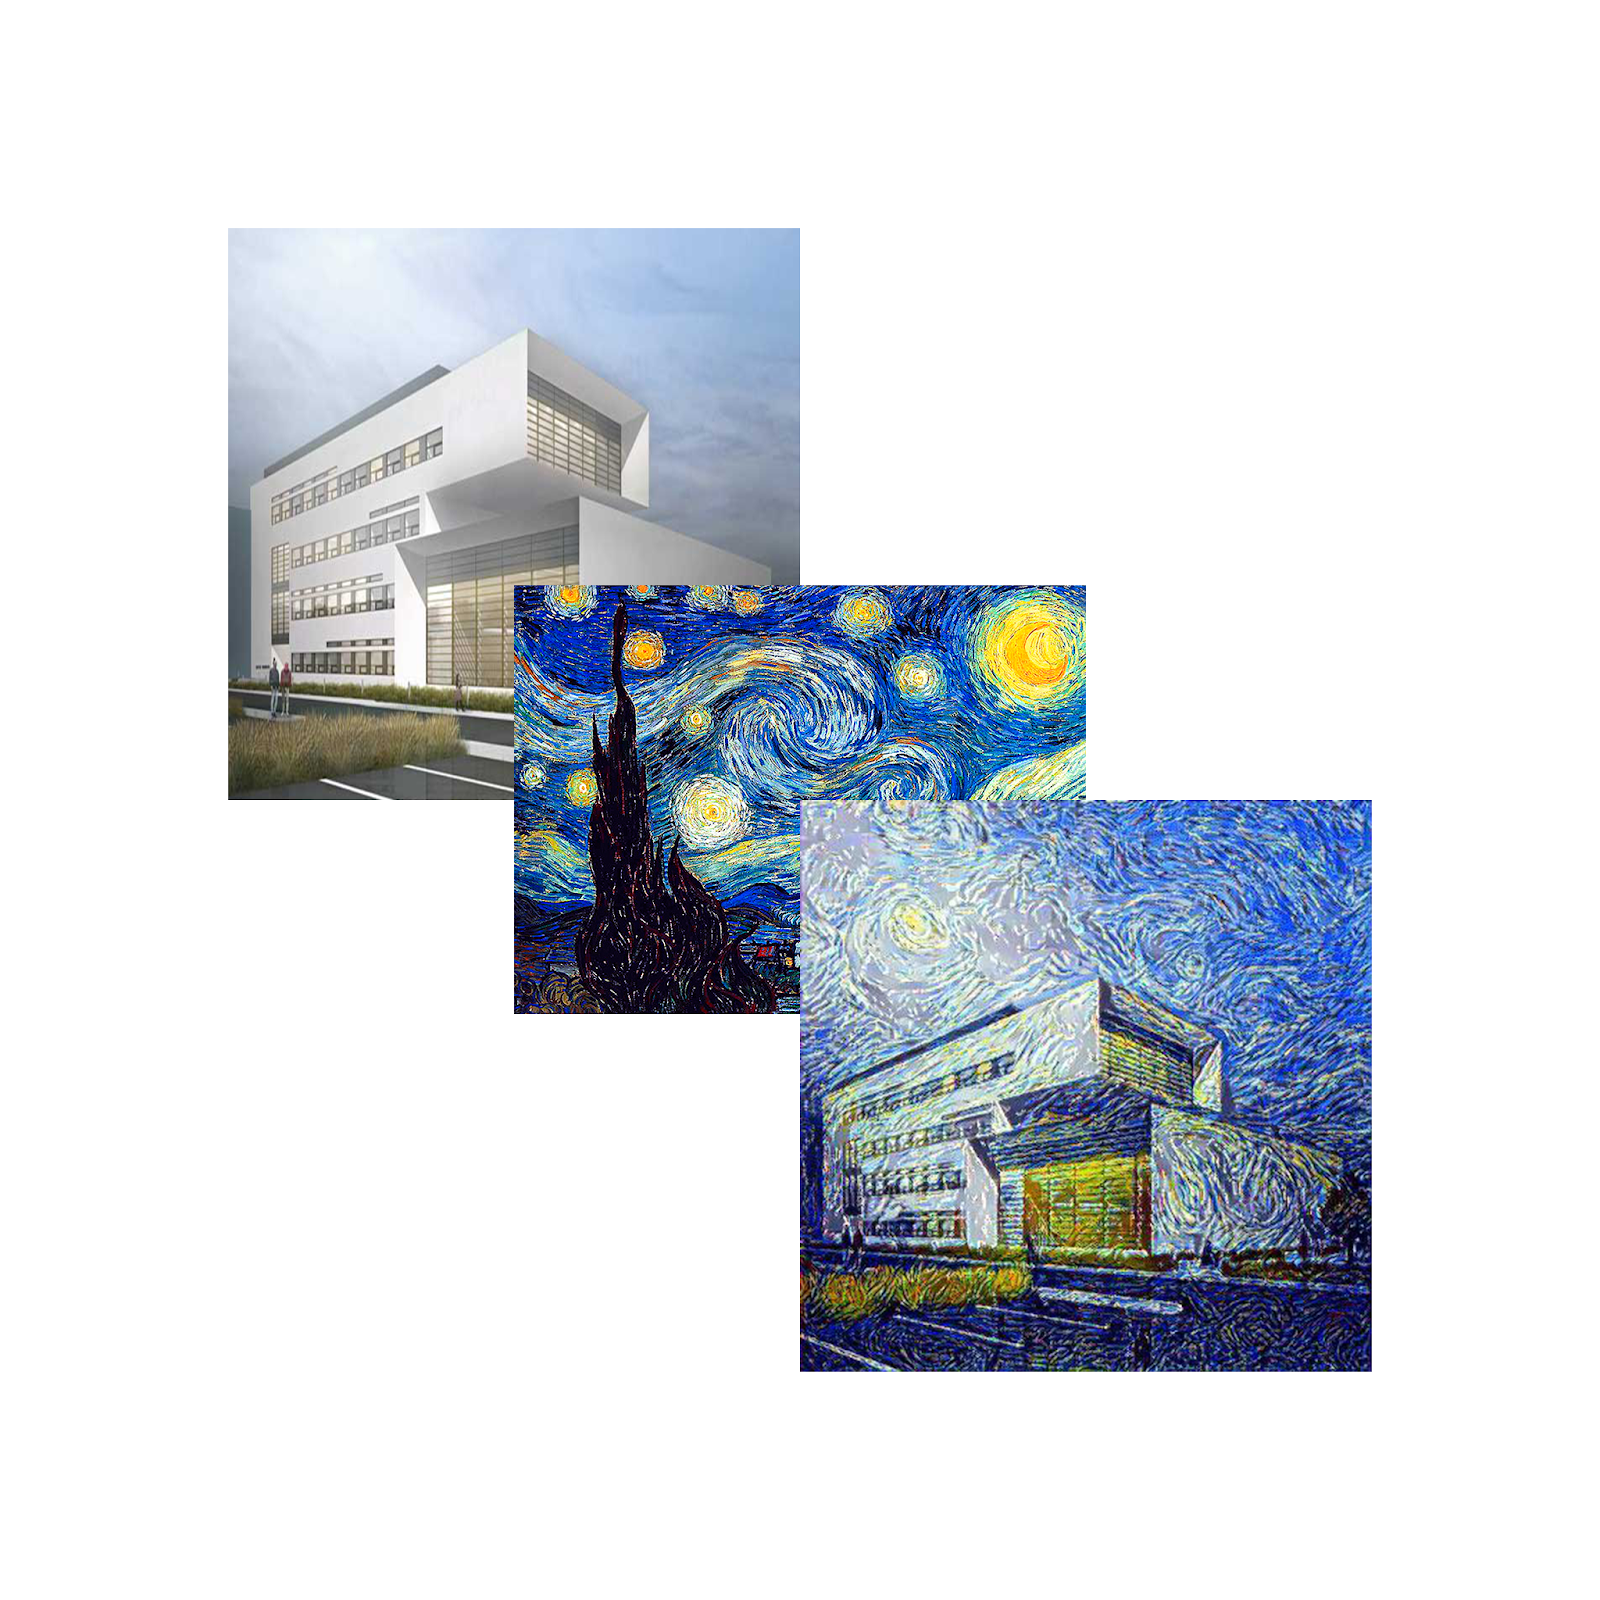
\includegraphics[width=.8\hsize]{fig/6}
\caption{Przykład zastosowania tranferu stylu
Obrazy łączące treść zdjęcia ze stylem kilku znanych dzieł sztuki. Obrazy zostały utworzone przez znalezienie obrazu, który jednocześnie pasuje do reprezentacji treści fotografii i stylu kompozycji. Oryginalne zdjęcie przedstawiające wizualizację nowego budynku wydziału Informatygi UIniwersytetu Gdańskiego. Obraz, który zapewnił styl dla odpowiedniego wygenerowanego obrazu, Gwiaździsta noc Vincenta van Gogha, 1889. Na samym końcu widzimy obraz wyjścia po wykonianiu 2048 iteracji(więcej o iteracjach w rodziale Inplementacja).
\label{RYS.6}}
\source{Opracowanie własne}
\end{figure}

----------------literówki------------

Oddzielenie treści od stylu w  obrazach jest niezwykle trudnym problemem. Jednak ostatni postęp w głębokich konwolucyjnych sieciach neuronowych [4] stworzył potężne komputerowe systemy interpretacji obrazu, które uczą się wyodrębniać informacje semantyczne na wysokim poziomie z obrazów naturalnych.

Koncepcyjnie jest to algorytm przesyłania tekstur, który ogranicza metodę syntezy tekstur poprzez reprezentacje cech z supernowoczesnych sieci neuronowych konwergentnych.[4] Ponieważ model tekstury opiera się również na głębokich reprezentacjach obrazu, metoda transferu stylu elegancko ogranicza się do problemu optymalizacji w ramach jednej sieci neuronowej. Nowe obrazy są generowane przez wykonanie wyszukiwania przed obrazem w celu dopasowania reprezentacji cech przykładowych obrazów.

Kiedy konwolucyjne sieci neuronowe są szkolone w zakresie rozpoznawania obiektów, rozwijają reprezentację obrazu, która sprawia, że informacje o obiektach stają się coraz bardziej wyraźne wzdłuż hierarchii przetwarzania. Dlatego wzdłuż hierarchii przetwarzania sieci obraz wejściowy przekształca się w reprezentacje, które są coraz bardziej wrażliwe na rzeczywistą treść obrazu, ale stają się względnie niezmienne dla jego dokładnego wyglądu. Zatem wyższe warstwy w sieci wychwytują zawartość wysokiego poziomu w kategoriach obiektów i ich rozmieszczenia w obrazie wejściowym, ale nie ograniczają bardzo dokładnie wartości pikseli w rekonstrukcji. Natomiast rekonstrukcje z niższych warstw po prostu odtwarzają dokładne wartości pikseli oryginalnego obrazu Dlatego też opis funkcji w wyższych warstwach sieci nazywamy reprezentacją treści.


\section{Model\label{s:dsssl}}
Modelem określamy sieć neuronową z dopasowanymi wagami osiągającą wysoką skutecznś np. w przypadku klasyfikacji.

literówki. Wyjaśnij co to znaczy "trenować model"

Aby trenować model, potrzeba:

\begin{itemize}
\item źródła danych treningowych
\item optymalizatora do dostosowania modelu do danych treningowych 
\item pętli  
\item sposobu uzyskania modelu i danych sprzętu, które będą wykonywać obliczenia potrzebne do wyszkolenia modelu

\end{itemize}

Transfer stylu to bardzo złożona technika wymagająca bardzo złożonego wytrenowanego modelu. Tutaj przydatne okazują się wytrenowane już modele. VGG19 jest bardzo efektywny przy ekstrakcji cech.

\section{Matryca Gram\label{s:dsssl}}

literówki. Pojęcie "preprocesing" bez wyjaśnienia, użyłbym jakiegoś polskiego odpowiednika, żeby nie tłumaczyć. Potrzebne jest objaśnienie zmiennych we wzorach. I krótkie ich opisanie, bo aktualnie są wklejone trochę od czapy.

Jest to krok niezbędny aby osięgnąć efektywną jak i efektowną ekstrakcję stylu.

Wyciągnięty styl wciąż przecowuje informację niepotrzebne, takie jak pozycje elementów czy ich strukturę na obrazie trzeba to wyczyścić .
Trzeba wykonać preprocesing na macierzy cech, która została wyciągnięta.

\begin{equation}
Gram = V^TV
\end{equation}


\begin{equation}
gram\:=\:torch.mm (tensor,\:tensor.t)
\end{equation}




\section{VGG19\label{s:dsssl}}

VGG (ang. Visual Geometry Group) to pretrenowany model konwolucyjnej sieci neuronowej. 
Wytrenowana na uniwersytecie Oksfordzkim została powszechnie udostępniona. Została ona  przeszkolona w zakresie rozpoznawania i lokalizacji obiektówi jest szczegółowo opisana w oryginalnej pracy [5].

Rozpoznawania i lokalizacji obiektów gdzie? na obrazie?

\begin{figure}[!tbh]
\centering
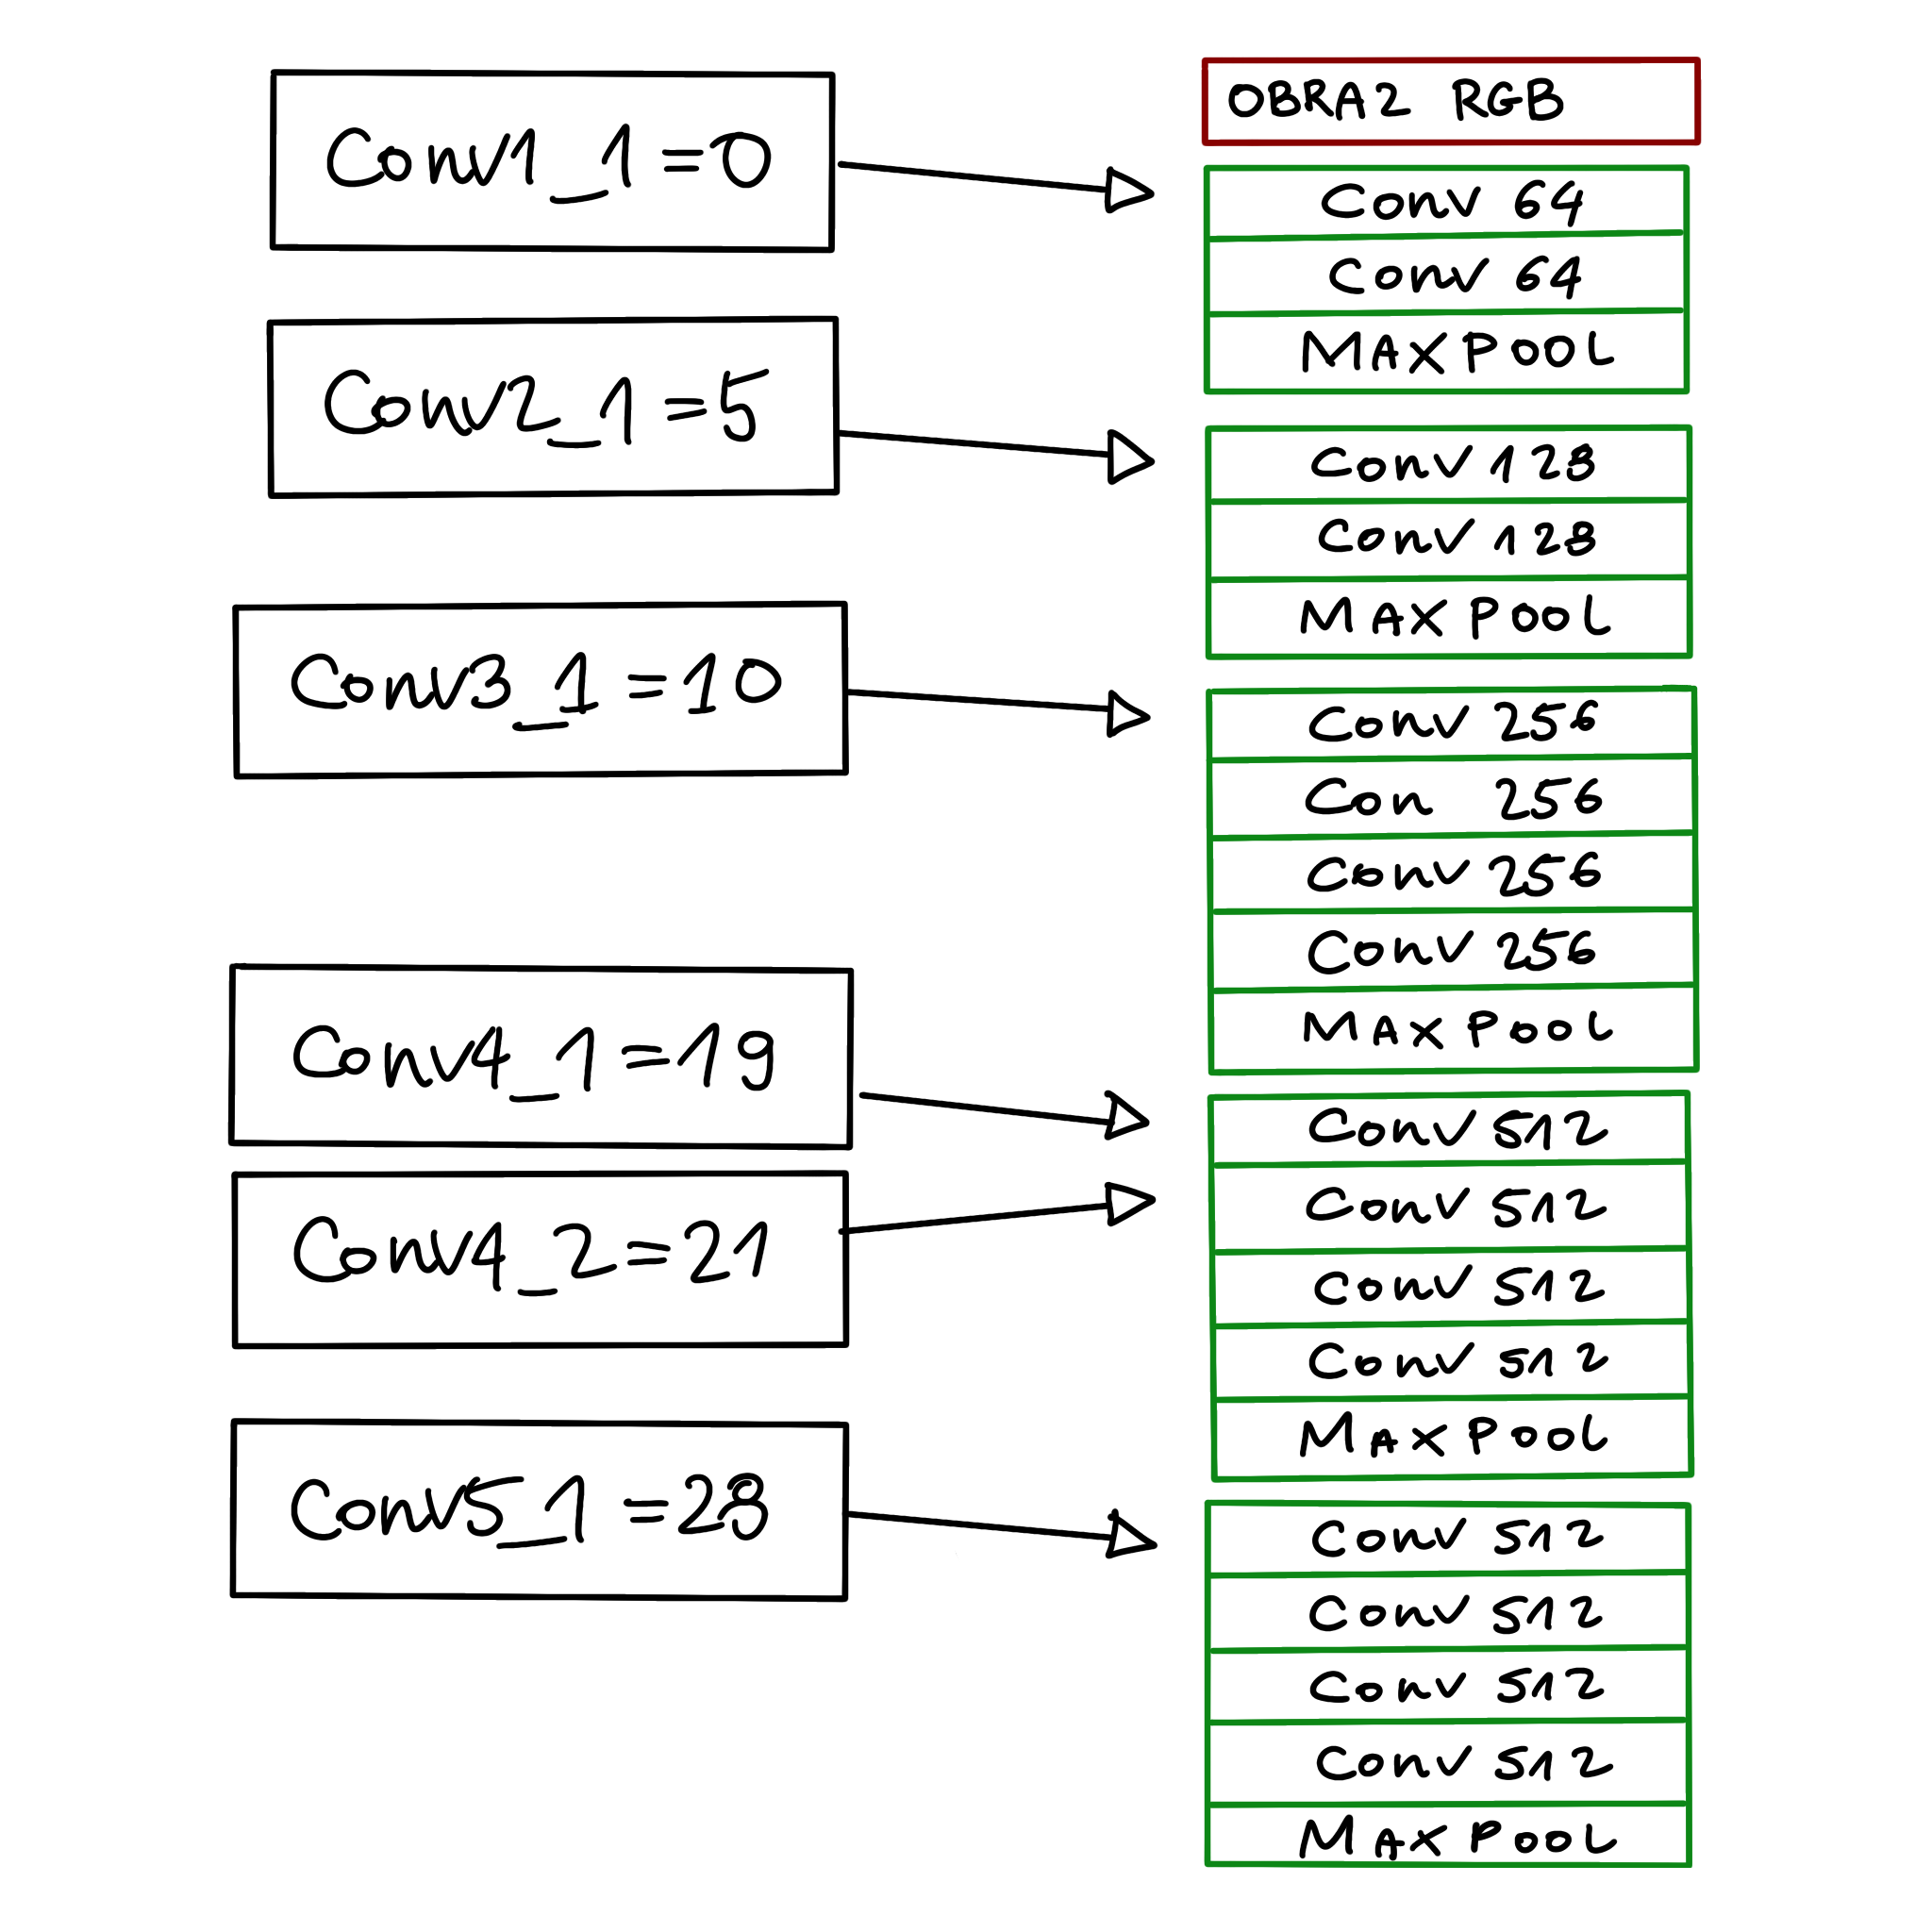
\includegraphics[width=.8\hsize]{fig/7}
\caption{Struktura VGG19\label{RYS.4}}
\source{Opracowanie własne}
\end{figure}


Kluczowe w tym przypaku jest klasyfikacja oraz wyodrębnianie funkcji.
VGG19 Wykorzystuje przestrzeń cech, jaką zapewnia znormalizowana wersja 16 konwojacyjnych i 5 warstw pulujących 19-warstwowej sieci VGG. Znormalizowaliśmy sieć, skalując wagi tak, aby średnia aktywacja każdego filtra splotowego względem obrazów i pozycji była równa jeden. Takie ponowne skalowanie można wykonać dla sieci VGG bez zmiany jej mocy wyjściowej, ponieważ zawiera ona jedynie prostujące liniowe funkcje aktywacyjne i nie ma normalizacji ani łączenia nad mapami cech. Nie używamy żadnej z w pełni połączonych warstw. Model jest publicznie dostępny. W przypadku syntezy obrazu stwierdzono, że zastąpienie maksymalnej operacji łączenia przez średnie łączenie w pulę daje nieco bardziej atrakcyjne wyniki, dlatego pokazane obrazy zostały wygenerowane ze średnim zestawieniem w puli. 

Wybieramy ktore warstwy w VGG19 używamy do znajdywania cech 
$def_features$

wszystkie warstwy wyciągają styl a tylko 21 wyciąga kontent

\begin{equation}
model.vgg19(pretrained=True)
\end{equation}

aby zachować stałe ustawienia parametrów i nie zmieniać ich przez wteczną propagację, co mogłoby popsuć model (overfitting)


To zdanie "Model jest publicznie dostępny" to trochę wtrącenie. Piszesz, co jest używane, a nagle wtrącenie o publiczności.

\begin{equation}
for\:param:\ in \: vgg.parameters():\:
	param.requires\_grad\_(False)
\end{equation}

objaśnienie do kodu.

\section{Szkolenie\label{s:dsssl}}

Na początku możliwe musi być analiza obrazu "stylu" i odzielenie stylu obrazka od jego zawartości. 
Następnym krokiem jest tranfer tego stylu z jednego obrazka do drugiego.

Aby przenieść styl kompozycji z jednego obrazka na drugi, syntezujemy nowy obraz, który jednocześnie pasuje do reprezentacji treści i reprezentacji stylu. W ten sposób wspólnie minimalizujemy odległość reprezentacji cechy białego szumu od reprezentacji treści zdjęcia w jednej warstwie oraz stylowej reprezentacji obrazu zdefiniowanej na kilku warstwach sieci neuronowej splotowej.

Reprezentacje treści i stylu w sieci neuronowej splotowej są dobrze rozdzielne. Oznacza to, że można niezależnie manipulować obiema reprezentacjami, aby wytwarzać nowe, sensownie postrzegalne obrazy. Aby zademonstrować to odkrycie, generujemy obrazy, które mieszają reprezentację treści i stylu z dwóch różnych obrazów źródłowych.

Innym ważnym czynnikiem w procesie syntezy obrazu jest wybór warstw pasujących do treści i reprezentacji stylu. Jak opisano powyżej, reprezentacja stylu jest reprezentacją wieloskalową, która obejmuje wiele warstw sieci neuronowej. Liczba i położenie tych warstw determinuje lokalną skalę, w której dopasowany jest styl, co prowadzi do różnych wrażeń wizualnych [4]. Zauważyliśmy, że dopasowanie reprezentacji stylu do wyższych warstw w sieci zachowuje struktury obrazów lokalnych na coraz większą skalę, co zapewnia płynniejsze i bardziej ciągłe wrażenia wizualne. Dlatego najbardziej atrakcyjne wizualnie obrazy są zwykle tworzone przez dopasowanie reprezentacji stylu do wysokich warstw w sieci, dlatego dla wszystkich wyświetlanych obrazów dopasowujemy cechy stylu na warstwach „conv1 1”, „conv2 1”, „conv3 1 ”,„ conv4 1 ”i„ conv5 1 ”sieci.

						
\section{Ograniczenia\label{s:dsssl}}

Prawdopodobnie najbardziej ograniczającym czynnikiem jest rozdzielczość zsyntetyzowanych obrazów. Zarówno wymiar problemu optymalizacji, jak i liczba jednostek w sieci neuronowej splotowej rosną liniowo wraz z liczbą pikseli. Dlatego szybkość procedury syntezy zależy w dużej mierze od rozdzielczości obrazu. Obrazy przedstawione w tym artykule zostały zsyntetyzowane w rozdzielczości około 512 × 512 pikseli, a procedura syntezy może zająć nawet godzinę na GPU Nvidia K40 (w zależności od dokładnego rozmiaru obrazu i kryteriów zatrzymania spadku gradientu). Podczas gdy ta wydajność obecnie zabrania stosowania online i interaktywnych aplikacji naszego algorytmu transferu stylu, prawdopodobne jest, że przyszłe ulepszenia w głębokim uczeniu również zwiększą wydajność tej metody.

- ----- czym jest sieć neuronowa splotowa?-------

Inną kwestią jest to, że zsyntetyzowane obrazy są czasami poddawane szumom o niskim poziomie. Chociaż jest to mniej problem w przypadku transferu stylu artystycznego, problem staje się bardziej widoczny, gdy zarówno treść, jak i obrazy w stylu są fotografiami i wpływa na fotorealizm zsyntetyzowanego obrazu. Jednak hałas jest bardzo charakterystyczny i wydaje się przypominać filtry jednostek w sieci. 

----Czym jest "hałas"? ------

Zatem możliwe byłoby skonstruowanie skutecznych technik usuwania szumów w celu późniejszego przetwarzania obrazów po procedurze optymalizacji.
Artystyczna stylizacja obrazów jest tradycyjnie badana w grafice komputerowej pod marką niefotorealistycznego wyrzeczenia. Oprócz pracy nad transferem tekstur, powszechnie stosowane podejścia różnią się koncepcyjnie od naszej pracy, ponieważ zapewniają wyspecjalizowane algorytmy do renderowania obrazu źródłowego w jednym określonym stylu. 

Oddzielenie treści obrazu od stylu nie jest koniecznie dobrze zdefiniowanym problemem. Wynika to głównie z tego, że nie jest jasne, co dokładnie określa styl obrazu. Mogą to być pociągnięcia pędzlem na obrazie, mapa kolorów, niektóre dominujące formy i kształty, ale także kompozycja sceny i wybór podmiotu obrazu - i prawdopodobnie jest to połączenie ich wszystkich i wiele więcej. Dlatego ogólnie nie jest jasne, czy treść obrazu i styl można w ogóle całkowicie oddzielić - a jeśli tak, to w jaki sposób. Na przykład nie jest możliwe renderowanie obrazu w stylu „Gwiaździstej nocy” van Gogha bez struktur obrazowych przypominających gwiazdy. W naszej pracy uważamy przeniesienie stylu za udane, jeśli wygenerowany obraz „wygląda” na styl, ale pokazuje obiekty i scenerię obrazu zawartości. Jesteśmy jednak w pełni świadomi, że to kryterium oceny nie jest ani matematycznie dokładne, ani uniwersalne.


\section{Podsumowanie\label{s:dsssl}}

System ten pozwala - przynajmniej w pewnym stopniu - na oddzielenie treści obrazu od stylu. Jednym z wyjaśnień może być to, że podczas uczenia się rozpoznawania obiektów sieć musi stać się niezmienna dla wszystkich odmian obrazu, które zachowują tożsamość obiektu. Reprezentacje, które uwzględniają zmienność treści obrazu i zmienność jego wyglądu, byłyby niezwykle praktyczne dla tego zadania. W świetle uderzających podobieństw między zoptymalizowanymi pod kątem wydajności sztucznymi sieciami neuronowymi a wizją biologiczną, kuszące jest spekulowanie, że ludzka zdolność do wyodrębniania treści ze stylu - a zatem nasza zdolność do tworzenia i ciesz się sztuką - może być również przede wszystkim znakiem rozpoznawczym potężnych możliwości wnioskowania naszego systemu wizualnego.


\chapter{Zakończenie}
Możliwości jaki stoją przed obrazami generowanymi maszynowo są nieograniczone zarówno do prototypowania i tworzenia "bazy" pomysłów, jak również do odciążania człowieka z zadań które jeszcze kilka lat temu były wykonalne tylko dla najlepszych specjalistów w branży.

Zakończenie powinno być przed bibliografią. Napisz co zostało pokazane w pracy, że podstawowe pojęcia dotyczące SI, sieci neuronowe, omówione zostały biblioteki. Po co zostały te rzeczy omówione. Że został pokazany transfer stylu, co pozwala, że zostały pokazane także jego ograniczenia. Jakie można podjąć kolejne kroki, aby usprawnić proces transferu stylu? (albo jakiś inny algorytm). 


\chapter{Bibliografia}

\begin{itemize}
\item$[1] Alan Turing, "Computing Machinery and Intelligence", 
Mind, vol. LIX, no. 236, Październik 1950$
\item$[2] Ian Goodfellow and Yoshua Bengio and Aaron Courville, 
"Deep Learning An MIT Press book", https://www.deeplearningbook.org$
\item $[3]Vishnu Subramanian Deep Learning with PyTorch https://arxiv.org/pdf/1508.06576.pdf $ 
\item $[4]Leon A. Gatys, Alexander S. Ecker, Matthias Bethge "A Neural Algorithm of Artistic Style" $
\item $[5]https://www.cv-foundation.org/openaccess/content_cvpr_2016/papers/Gatys_Image_Style_Transfer_CVPR_2016_paper.pdf$

\item $[6] Lemaréchal, C. (2012). "Cauchy and the Gradient Method" (PDF). Doc Math Extra: 251–254.$


\item $[7]https://papers.nips.cc/paper/5633-texture-syanthesis-using-convolutional-neural-networks.pdf$

\item$[8]K. Simonyan and A. Zisserman. Very Deep Con- volutional Networks for Large-Scale Image Recognition. arXiv:1409.1556 [cs], Sept. 2014. arXiv: 1409.1556.$
\item $[9]Grokking Deep Learning, by Andrew W. Trask$
\item $[10]Deep Learning with PyTorch by Eli Stevens and Luca Antiga$
\item $[11]Czysty kod. Podręcznik dobrego programisty Robert C. Martin$
\item $[12]https://pytorch.org/tutorials/advanced/neural_style_tutorial.html$
\item $[13]https://github.com/rrmina/neural-style-pytorch$
\item $[14]https://polycount.com/discussion/205872/creating-images-with-python-in-blender$
\item $[15]https://cloud.blender.org/p/scripting-for-artists/5993ed908119170ebb57164b$
\item $[16]https://www.3blue1brown.com$
\item $[17]https://www.manning.com/books/grokking-deep-learning$
\item $[18]https://www.deeplearningbook.org$
\item $[19]Deep Learning, by Ian Goodfellow, Yoshua Bengio, and Aaron Courville.$


\end{itemize}


% załączniki (opcjonalnie):
\appendix
\chapter{Tytuł załącznika jeden}

Treść załącznika jeden.

\chapter{Tytuł załącznika dwa}

Treść załącznika dwa.

% literatura (obowiązkowo):
\bibliographystyle{unsrt}
\bibliography{xml}


\oswiadczenie

\end{document}
